

\chapter{Numerical Methods}


\section{Numerical Hydrodynamics}

Consider the 1D advection equation

\begin{equation}
\frac{\partial f}{\partial t} = -u\frac{\partial f}{\partial x}
\end{equation}

and let us discretize it in time and space. There are different ways
we can approximate the spatial derivative

\beqn
\frac{\partial f}{\partial x} &\approx& \frac{f_i -
  f_{i-1}}{\Delta x} \quad \mathrm{FTBS \ forward \ time \ back \ space}\\
\frac{\partial f}{\partial x} &\approx& \frac{f_{i+1} -  f_i}{\Delta  x} \quad \mathrm{FTFS \ forward \ time \ foward \ space}\\
\frac{\partial f}{\partial x} &\approx& \frac{f_{i+1} -  f_{i-1}}{2\Delta x}\quad \mathrm{FTBS \ forward \ time \ center \ space}\\
\frac{\partial f}{\partial x} &\approx& \frac{f_{i+1/2} - f_{i-1/2}}{\Delta x}
\eeqn


Let us pick the centered 

\begin{equation}
\frac{f^{(n+1)}_i - f^{(n)}_i}{\Delta t } = - u \left( \frac{f^{(n)}_{i+1} - f^{(n)}_{i-1}}{2\Delta x}\right)
\end{equation}


We isolate the quantity we want to find, $f_i$ in the future

\begin{equation}
f^{(n+1)}_i  = f^{(n)}_i - \frac{u\Delta t}{2\Delta x} \left( f^{(n)}_{i+1} - f^{(n)}_{i-1}\right)
\end{equation}

We define the {\bf Courant number}, which is a dimensionless quantity
that, as we see later, determines the {\it stability} of the different schemes

\begin{equation}
\boxed{
C \equiv \frac{u\Delta t}{\Delta x}
}
\end{equation}

In terms of the Courant number, the recurrence relation is 
\begin{equation}
f^{(n+1)}_i  = f^{(n)}_i - \frac{C}{2} \left( f^{(n)}_{i+1} - f^{(n)}_{i-1}\right)
\end{equation}


\subsection{Stencil Diagrams}

The field $f_i^{(n+1)}$ at grid point $i$ and time step $n + 1$
depends on values at the old time step $n$. This is sketched in a
so-called {\it stencil diagram}. 

\begin{figure}
  \begin{center}
    \resizebox{\textwidth}{!}{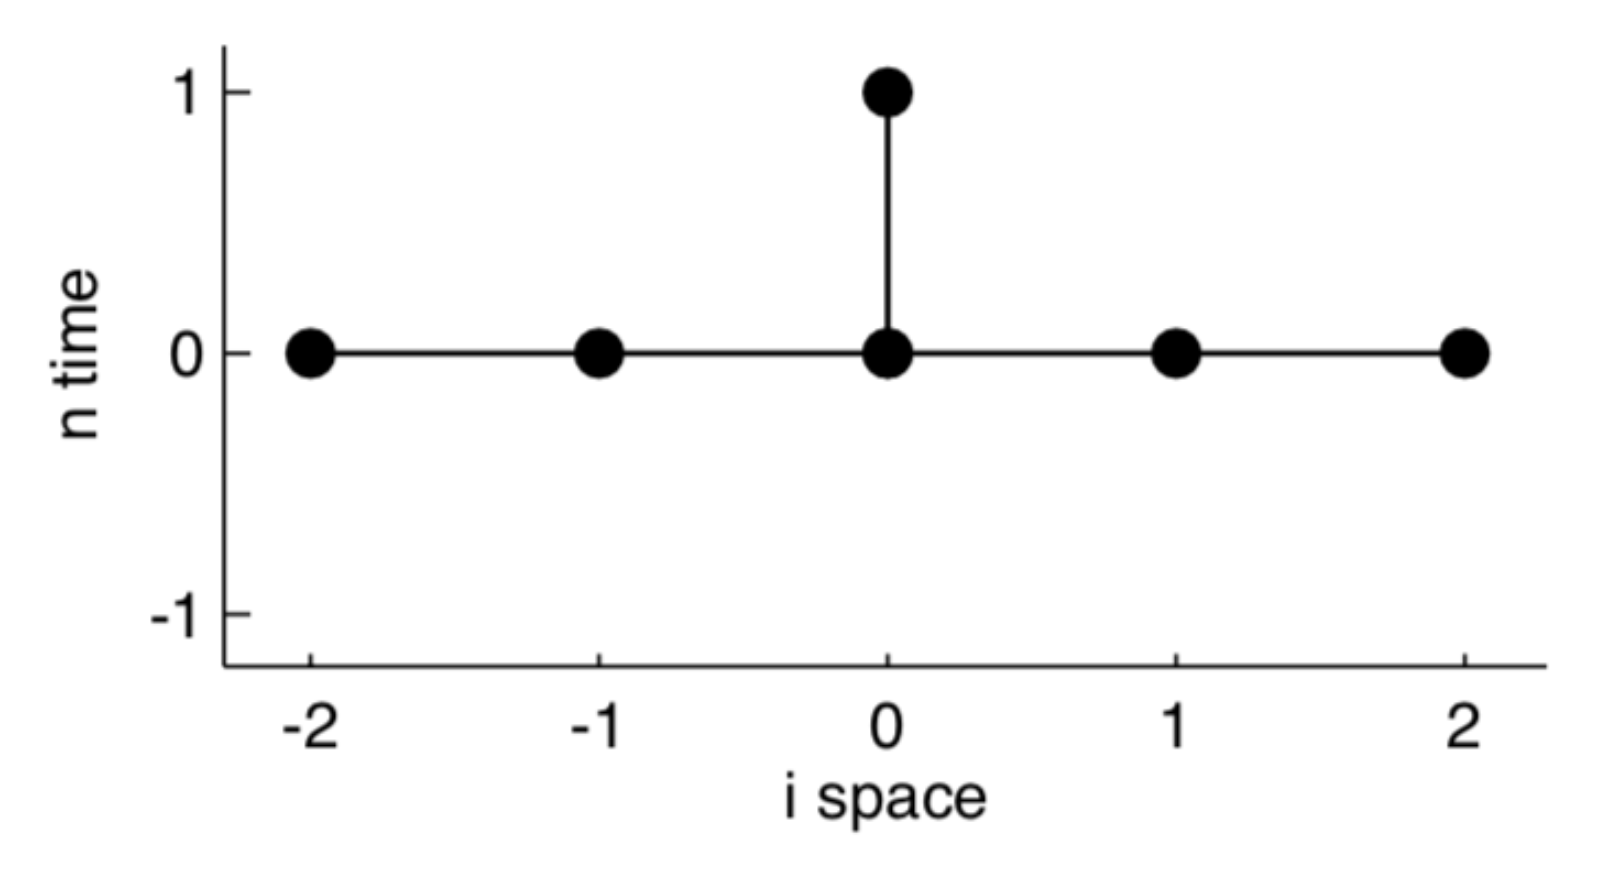
\includegraphics{./figs/stencil1.png}}
  \end{center}
  \caption[]{Stencil diagram}
  \label{fig:stencil1}
\end{figure}

\subsection{``Naive'' scheme}

%The ``naive'' scheme averages the adjacent grid points 

%\begin{equation}
%f_{i+1/2} = \frac{v}{2}\left(\rho_{i+1} + \rho_i\right)
%\end{equation}

%Leading to 

Consider the equation we obtained 

\begin{equation}
f^{(n+1)}_i  = f^{(n)}_i - \frac{C}{2}\left(f_{i+1} - f_{i-1}\right)
\end{equation}


\begin{figure}
  \begin{center}
    \resizebox{\textwidth}{!}{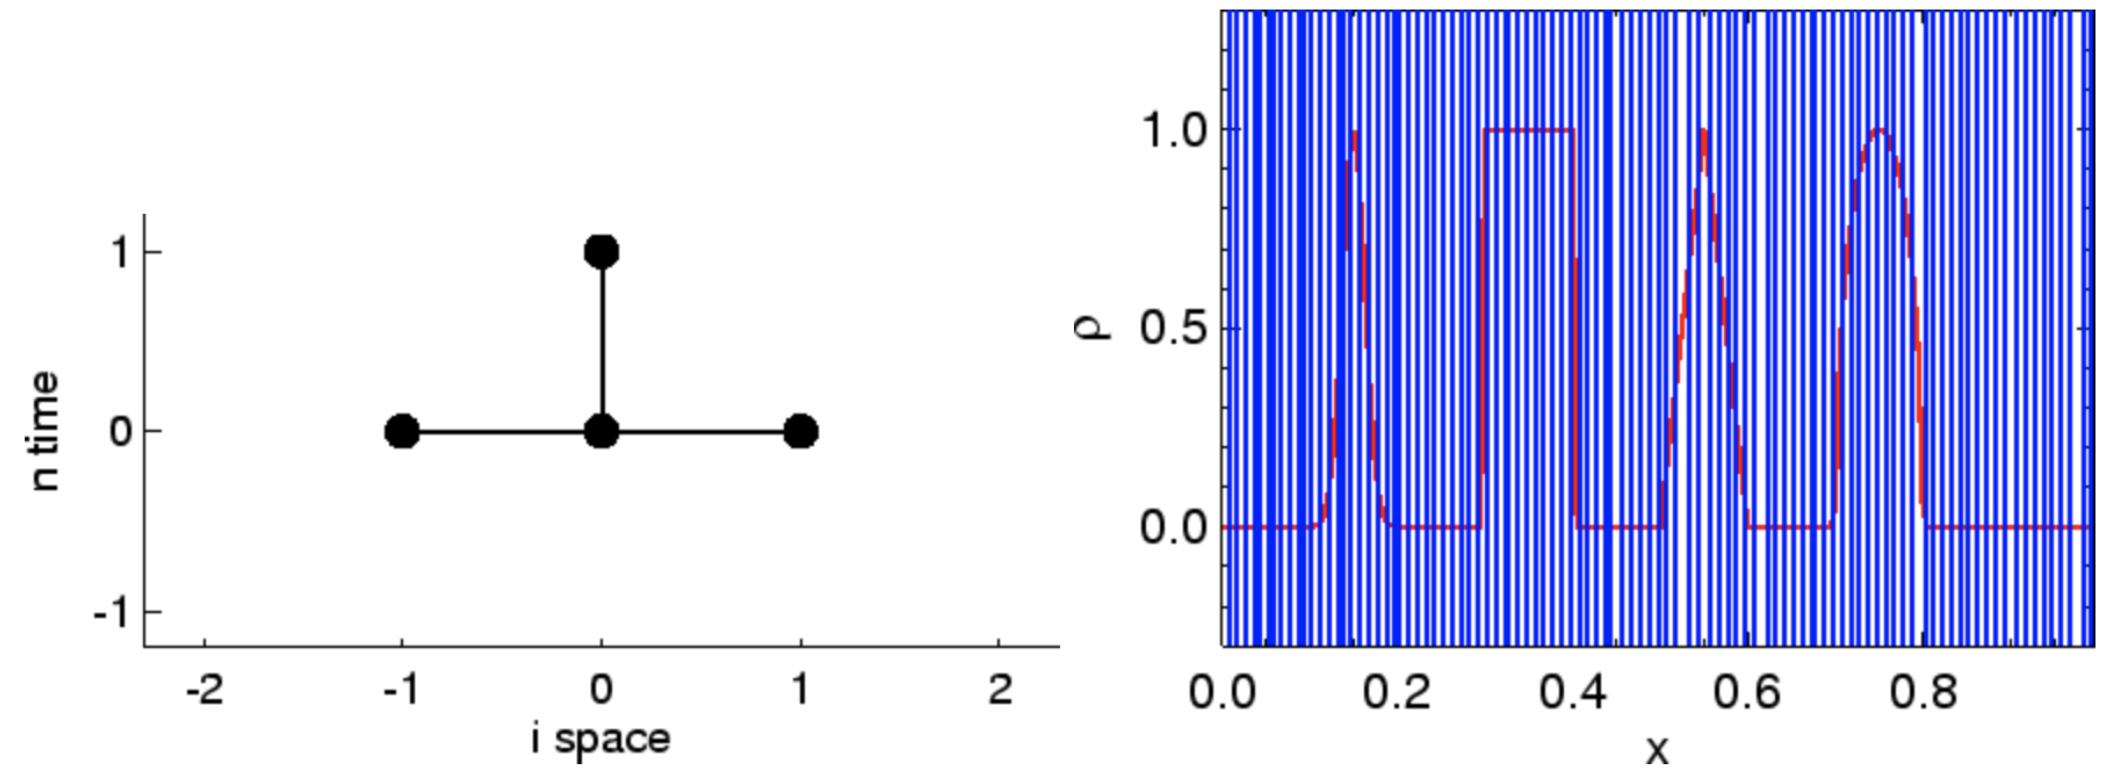
\includegraphics{./figs/naive.png}}
  \end{center}
  \caption[]{Centered difference ``naive'' scheme}
  \label{fig:naive-adv}
\end{figure}


The solution is shown in \fig{fig:naive-adv}. The oscillations are
seen to grow exponentially \figp{fig:naive-adv}. After some time the
numerical result does not have the faintest resemblance to true
solution. We will call this scheme ``naive''. 

\subsection{Von-Neumann stability analysis}

Why does the naive scheme fail so drastically? Let us look at a Fourier mode of the function

\begin{equation}
f(x,t) = A(t) e^{-ikx}
\end{equation}


The naive scheme turns into

\begin{equation}
A(t+\Delta t)e^{-ikx} = A(t)e^{-ikx} - \frac{C}{2}A(t)\left[e^{-ik(x+\Delta x)} - e^{-ik(x-\Delta x)}\right]
\end{equation}

multiplying by $e^{ikx}$


\begin{equation}
A(t+\Delta t) = A(t) \left[ 1 - \frac{C}{2}\left(e^{-ik\Delta x} -  e^{ik\Delta x}\right)\right]
\end{equation}

the term in parentheses in the RHS is the sine function

\classcomm{If class doesn't recognize it as the sin function, show quickly using Euler formula
  \beqn
  e^{ix}  &=& \cos x + i \sin x\\
  e^{-ix}  &=& \cos x - i \sin x\\
  \eeqn
  which leads to
  \beqn
  \cos x &=& \frac{e^{ix} + e^{-ix}}{2}\\
  \sin x &=& \frac{e^{ix} - e^{-ix}}{2i}\\
  \eeqn
}
  

\begin{equation}
A(t+\Delta t) = A(t)\left[1 + i C \sin \left(k\Delta x\right)\right]
\end{equation}

multiplying by the complex conjugate we find the amplitude

\begin{equation}
A^2(t+\Delta t) = A^2(t)\left[1 + C^2 \sin^2\left(k\Delta x\right)\right]
\end{equation}

We see that the amplitude of any wave, irrespective of $k$, will always increase, independently of the Courant number. The scheme is unconditionally unstable. 

\subsection{Back space (upwinding)}

\begin{figure}
  \begin{center}
    \resizebox{\textwidth}{!}{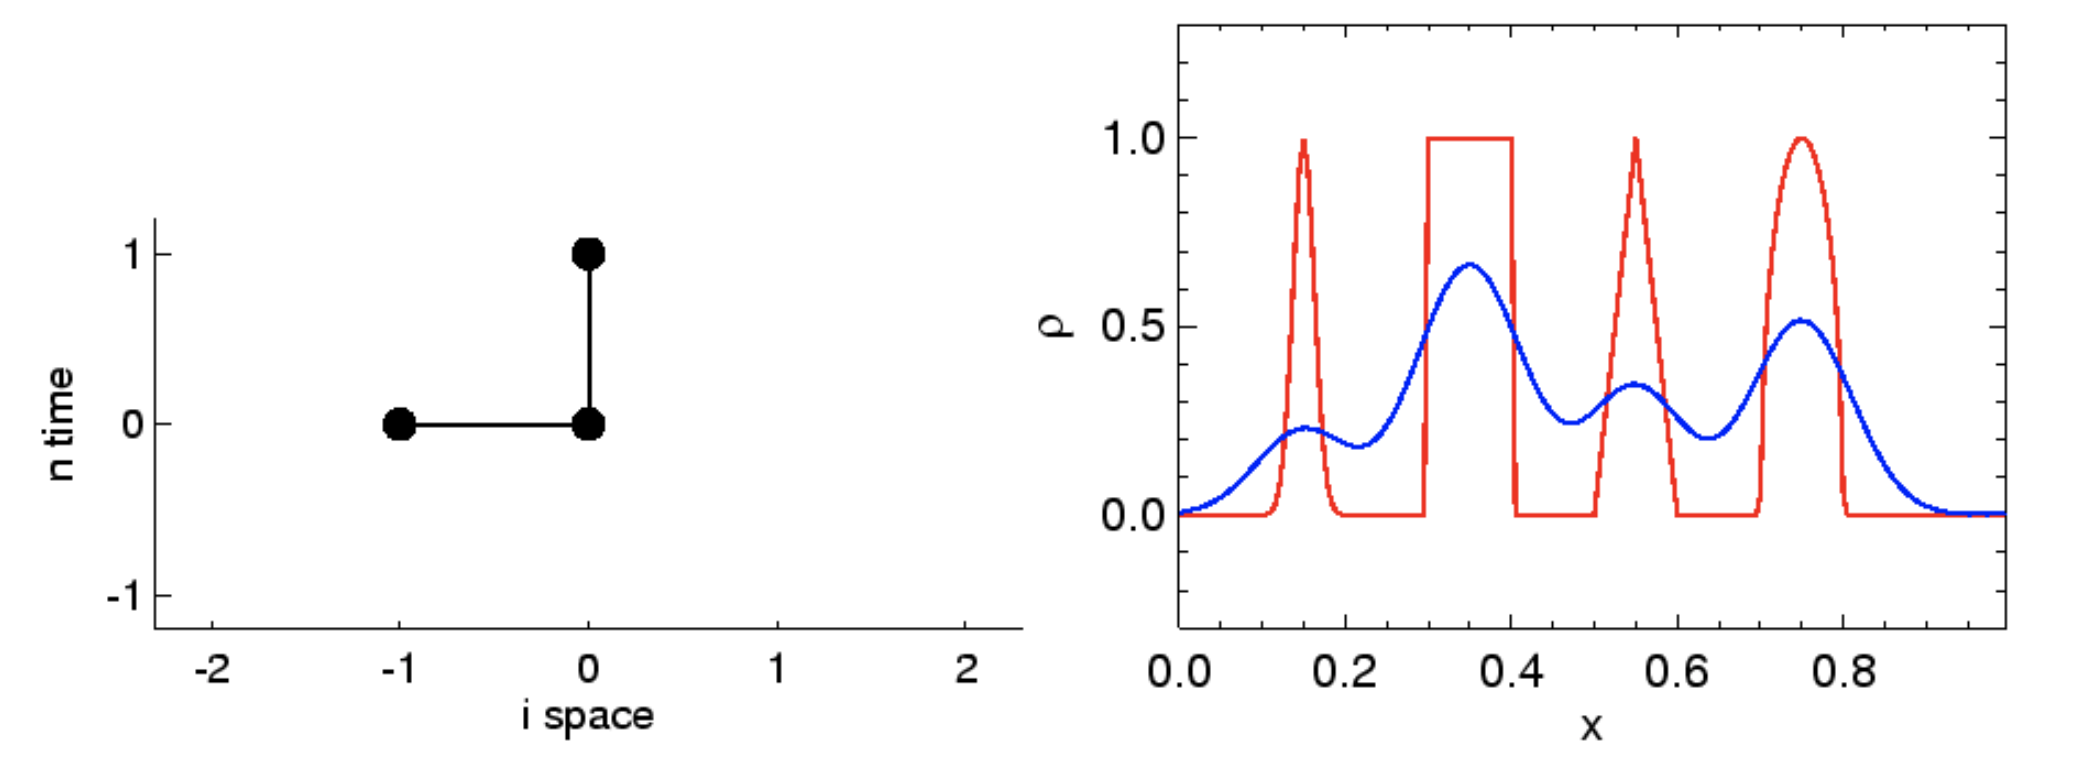
\includegraphics{./figs/donor.png}}
  \end{center}
  \caption[]{Donor cell}
  \label{fig:donor}
\end{figure}

The back space scheme uses the point upwind
(back space) for the derivative. The scheme results in 

\begin{equation}
f^{(n+1)}_i  = (1-C) f^{(n)}_i + Cf^{(n)}_{i-1}
\end{equation}

The stencil is sketched in \fig{fig:donor}. It depends on the point and the point immediately upwind. The Courant number is the weight given to the upwind point. 

The result is smooth but smeared out severely. Let us look at the von Neumann stability analysis upwind scheme. Using again a single Fourier mode 


\begin{equation}
f(x,t) = A(t) e^{-ikx}
\end{equation}

The upwind scheme turns into

\begin{equation}
A(t+\Delta t)e^{-ikx}  = (1-C) A(t)e^{-ikx} + CA(t)e^{-ik(x-\Delta x)}
\end{equation}

multiplying by $e^{ikx}$

\begin{equation}
A(t+\Delta t)  = A(t) \left(1 - C  +C e^{ik\Delta x}\right)
\end{equation}


expaning the exponential 

\begin{equation}
A(t+\Delta t)  = A(t) \left(1 - C + C\cos k\Delta x + C i\sin k\Delta x\right)
\end{equation}

Replacing $B = 1 - C + C\cos k\Delta x$ and $D = C\sin k\Delta x$

\begin{equation}
A(t+\Delta t)  = A(t) \left(B + iD\right)
\end{equation}

multiplying by the complex conjugate 

\begin{equation}
A^2(t+\Delta t)  = A^2(t) \left(B^2  + D^2\right)
\end{equation}

where the amplification factor is 

\begin{eqnarray}
B^2+D^2 &=& \left(1 - C + C\cos k\Delta x\right)^2 + C^2\sin^2 k\Delta x\\
&=&(1-C)^2 + 2(1-C)C\cos k\Delta x 
\end{eqnarray}


The maximum and minimum values of $\cos k\Delta x$ are 1 and -1, so the amplification is bound between 

\begin{equation}
(1-C)^2 - 2(C-C^2) \leq B^2+D^2 \leq (1-C)^2 + 2(C-C^2) 
\end{equation}

For the maximum amplification to be below 1 we require 

\begin{equation}
0 \leq 1 - C^2 \leq 1 
\end{equation}

which is true for 

\begin{equation}
\boxed{
C \leq 1
}
\end{equation}

This is the {\it condition of stability} of the upwind scheme.

Upwinding seems promising to achieve stability. However, the accuracy
of the scheme has to be improved.

Note on the nature of the ``smoothing'' of the solution. Even though
the advection equation does not have any diffusion in it, the
numerical algorithm to solve this advection equation intrinsically has
some diffusion. In fact, there exists no numerical method without
numerical diffusion. Some algorithms have more of it, some have less,
and there exist method to constrain the smearing-out of
discontinuities. But in principle numerical diffusion is
unavoidable.

One way of seeing this is by doing the following exercise. Consider the upwind scheme. It
uses the derivative $i- 1/2$ for the update of the state at $i$. So let us write the derivative at $i- 1/2$ as:

\beq
\frac{f_i-f_{i-1}}{\Delta x} = \frac{q_{i+1}-q_{i-1}}{2\Delta x} -
\Delta x \frac{f_{i+1}-2f_i+f_{i-1}}{2\Delta x^2}
\eeq

The left-hand-side is the upstream difference, the first term on the
right-hand-side is the centered difference and the second term on the
right-hand-side can be recognized as a diffusion term with diffusion constant

\beq
D=\frac{u\Delta x}{2}
\eeq

This shows that the upstream difference scheme can be regarded to be the same as the centered
difference scheme supplemented with a diffusion term. The pure centered difference scheme
is unstable, but once a bit of diffusion is added, the algorithm stabilizes. The drawback is,
however, that the diffusion smears any features out. If one would define the centered difference
formulation of the x-derivative as the ``true'' derivative (which is of course merely a definition),
then the numerical diffusion of the upstream differencing scheme is
quantified by D as given in the equation above. 

In practice it is not possible to perfectly define the diffusivity of an algorithm since the
centered difference formulation of the derivative is also merely an approximation of the true
derivative. But it is nevertheless a useful way of looking at the concept of numerical diffusion.
In principle one could say that it is as if we are solving

\beq
\frac{\partial f}{\partial t} = - u \frac{\partial f}{\partial x} +\frac{u\Delta x}{2}\frac{\partial^2 f}{\partial^2 x}
\eeq

Clearly, for $\Delta x \rightarrow 0$ the diffusion vanishes. This is obviously a necessary condition, otherwise
we would be modeling the true diffusion equation, which is not what we want. The diffusion
that we see here is merely a by-product of the numerical algorithm we
used. Note that sometimes (as we shall see below) it is useful to add
some viscosity on purpose to an algorithm. This is called artificial
viscosity. One could therefore say that the upstream differencing is equal to centered differencing plus artificial viscosity.

\section{Taylor series}

Taylor series are  expansions of a function $f(x)$ for some 
finite distance $\Delta x$ to $f(x+\Delta x)$

\beq
f(x\pm \Delta x) = f(x) \pm \Delta x f^\prime(x) + \frac{\Delta
  x^2}{2} f^{\prime\prime}(x) \pm \frac{\Delta x^3}{3!}
f^{\prime\prime\prime}(x) + \frac{\Delta
  x^4}{4!} f^{\prime\prime \prime\prime}(x) \pm ...
\eeq

What happens, if we use this expression for the forward derivative

\beq
\frac{\partial f}{\partial x} \approx \frac{f(x+\Delta x) - f(x)}{\Delta x}
\eeq

which leads to

\beqn
\frac{f(x+\Delta x) - f(x)}{\Delta x} &=& \frac{1}{\Delta x} \left[ \Delta x f^\prime(x) + \frac{\Delta
  x^2}{2} f^{\prime\prime}(x) + \frac{\Delta x^3}{3!}
f^{\prime\prime\prime}(x)\right]\\
&=&f^\prime(x) + \mathcal{O}\left(\Delta x\right)
\eeqn

The error of the first derivative using the forward 
formulation is of order $\Delta x$. Is this the case for other formulations of the derivative?
Let’s check.

With the centered formulation we get:

\beqn
\frac{f(x+\Delta x/2) - f(x-\Delta x/2)}{\Delta x} &=&\frac{1}{\Delta
  x} \left[ \Delta x f^\prime(x) + \frac{\Delta
    x^2}{3!}f^{\prime\prime\prime}(x)+...\right]\\
&=&f^\prime(x) + \mathcal{O}(\Delta x^2)
\eeqn

The error of the first derivative using the centered 
approximation is of order $\Delta x^2$. This is an important result: it does matter which formulation
we use. The centered scheme is more accurate. Yet, we just saw that
the more accurate one is unstable, whereas the less accurate one is
stable. {\it Accuracy does not guarantee stability.}

\section{High-order finite-difference derivatives}

The first derivative, to 2nd order accuracy is 

\begin{equation}
f_i^\prime = \frac{-f_{i-1} + f_{i+1}}{2\Delta x} + \mathcal{O}(\Delta x^2)
\end{equation}

to 4th order accuracy, it is 

\begin{equation}
f_i^\prime = \frac{f_{i-2} -8f_{i-1} +8f_{i+1} - f_{i+2}}{12\Delta x} + \mathcal{O}(\Delta x^4)
\end{equation}

to 6th order accuracy, it is 

\begin{equation}
f_i^\prime = \frac{-f_{i-3} + 9f_{i-2} -45f_{i-1} +45f_{i+1} -9f_{i+2} + f_{i+3}}{60\Delta x} + \mathcal{O}(\Delta x^6)
\end{equation}

The table shown in \fig{fig:tablecoefficients} shows the coefficients (weights) given to each point on computing a derivative to desired accuracy. We will draw from this table to compute first and second derivatives, mostly. But how are these coefficients determined?  

\begin{figure}
  \begin{center}
    \resizebox{\textwidth}{!}{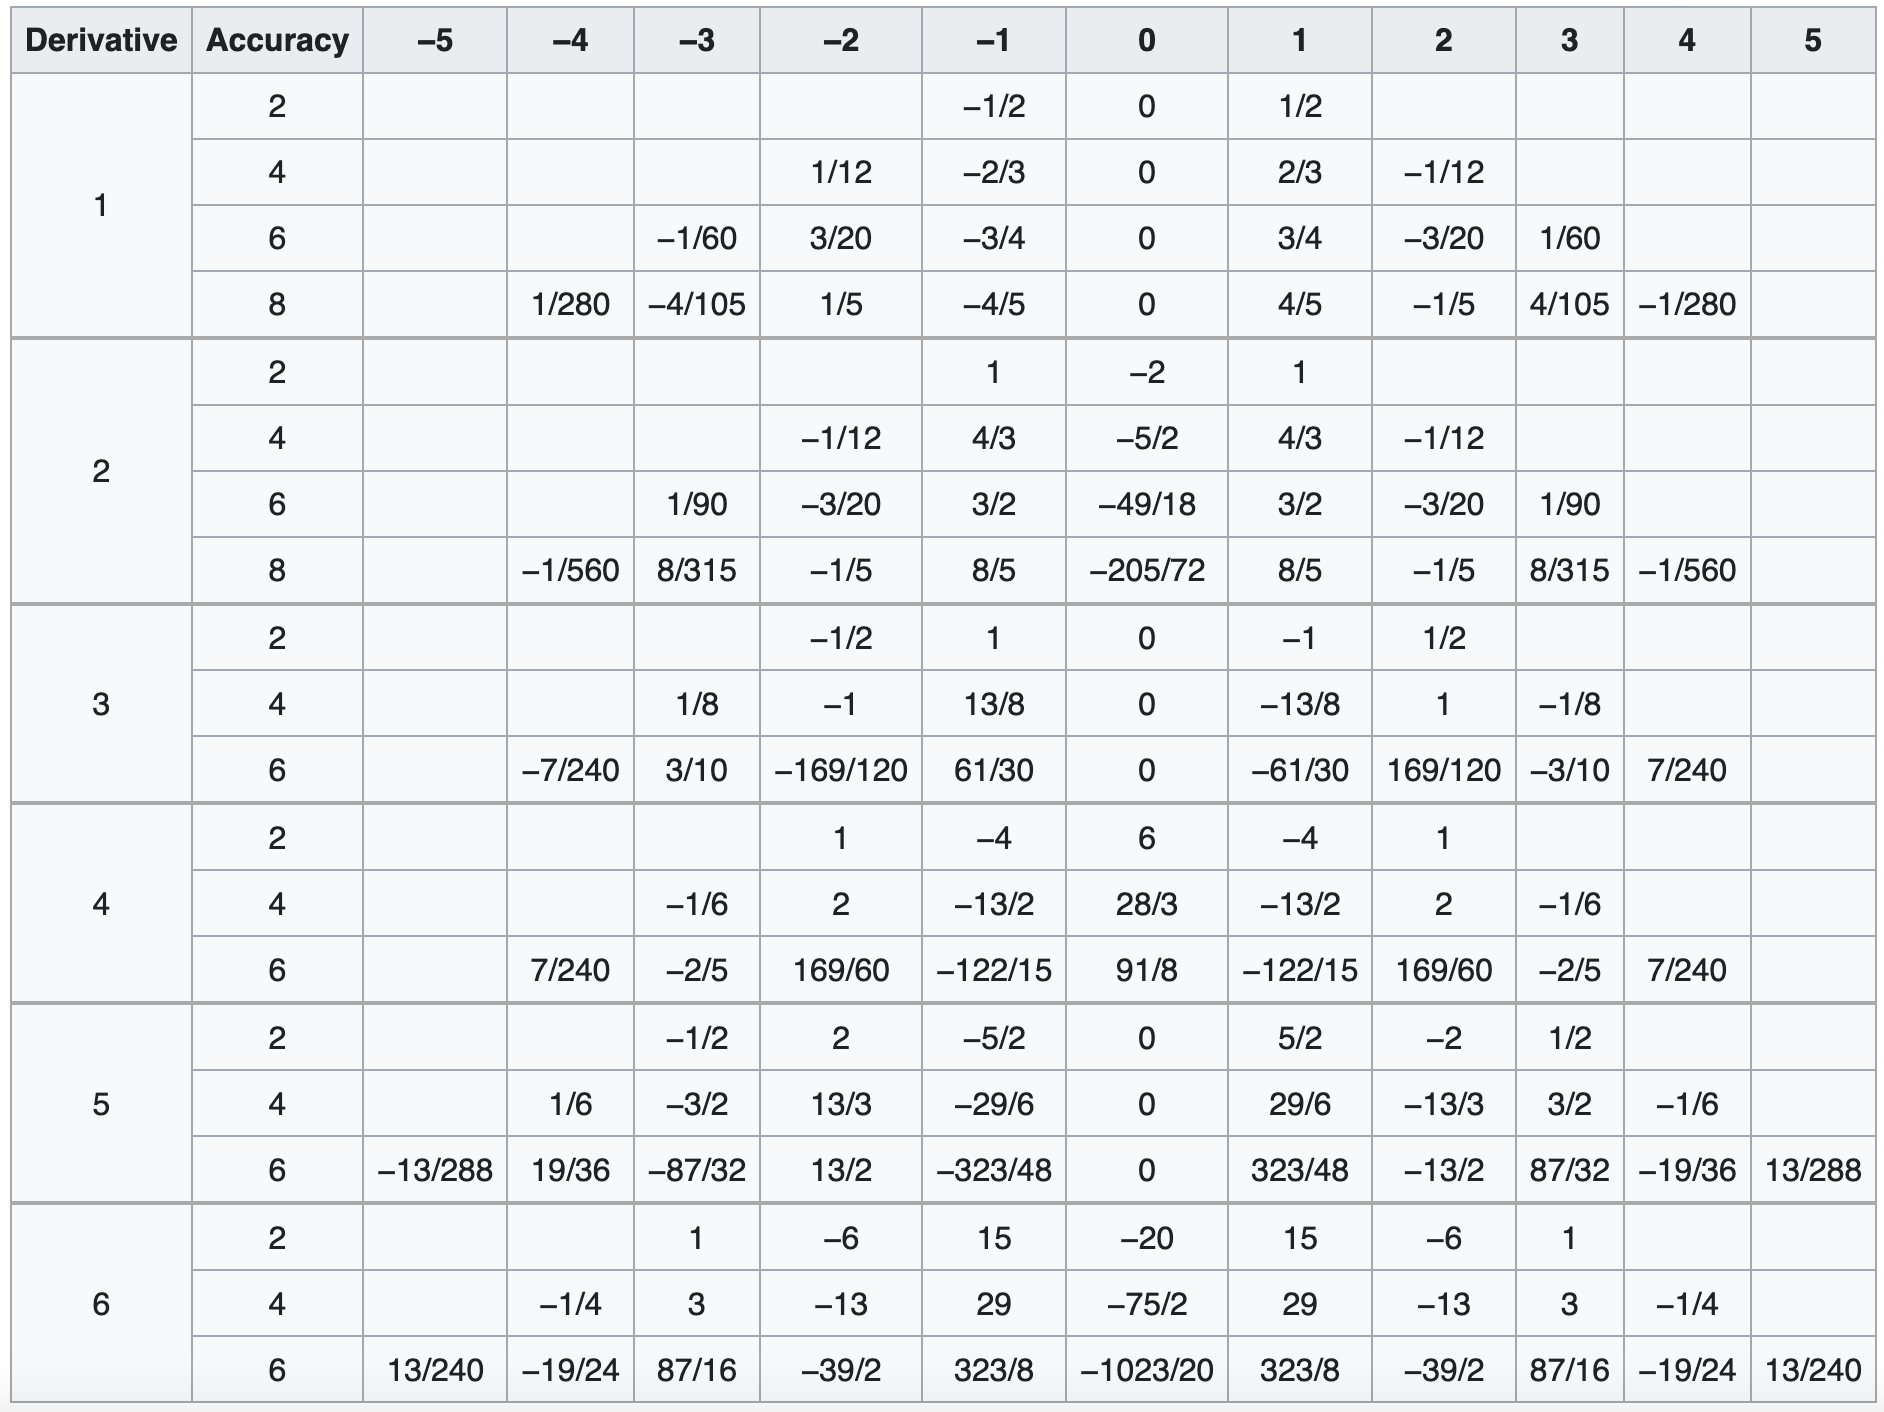
\includegraphics{./figs/tablecoefficients.png}}
  \end{center}
  \caption[]{}
  \label{fig:tablecoefficients}
\end{figure}

These coefficients come from Taylor expansion. Suppose that we want to compute df/dx to 2nd order. Using a 3-point stencil, we have 

\begin{equation}
\frac{df}{dx} = \frac{1}{h}\left[Af(x-h) + Bf(x) + Cf(x+h)\right]
\end{equation}

where $h=\Delta x$. According to the table in \fig{fig:tablecoefficients}, we expect to find $A=-1/2$, $B=0$ and $C=1/2$. Let us prove this.

If we Taylor expand around $x$, 

\begin{eqnarray}
Af(x-h) &=& Af(x) + Af^\prime(x)(-h) + Af^{\prime\prime}(x)\frac{h^2}{2}  \\
Bf(x)   &=& Bf(x)   \\
Cf(x+h) &=& Cf(x) + Cf^\prime(x)(h) + Cf^{\prime\prime}(x)\frac{h^2}{2} 
\end{eqnarray}

Summing them all 

\begin{equation}
h\frac{df}{dx} = f(x)(A+B+C) + f^\prime(x)(A-C)h + f^{\prime\prime}(x)\frac{h^2}{2}(A+C) 
\end{equation}

Since only the first derivative should survive in the RHS, this leads to the conditions 

\begin{eqnarray}
A+B+C&=&0\\
A-C &=& 1\\
A+C &=& 0 
\end{eqnarray}

Leading to $A=-1/2$, $C=1/2$, $B=0$, as expected.


Another example, find the fourth derivative $d^4f/dx^4$, with a 5-point stencil 


\begin{equation}
h^4\frac{d^4f}{dx^4} = Af(x-2h) + Bf(x-h) + Cf(x) + Df(x+h) + Ef(x+2h)
\end{equation}

Expanding the terms in Taylor to fourth order 

\begin{eqnarray}
Af(x-2h) &=& Af(x) + Af^\prime(x)(-2h) + Af^{\prime\prime}(x)\frac{(2h)^2}{2}  + Af^{\prime\prime\prime}(x)\frac{(-2h)^3}{6}+ Af^{\prime\prime\prime\prime}(x)\frac{(2h)^4}{24}\nonumber\\
Bf(x-h) &=& Bf(x) + Bf^\prime(x)(-h) + Bf^{\prime\prime}(x)\frac{h^2}{2}  + Bf^{\prime\prime\prime}(x)\frac{(-h)^3}{6}+ Bf^{\prime\prime\prime\prime}(x)\frac{h^4}{24}\nonumber\\
Cf(x) &=& Cf(x) \\
Df(x+h) &=& Df(x) + Df^\prime(x)(h) + Df^{\prime\prime}(x)\frac{h^2}{2}  + Df^{\prime\prime\prime}(x)\frac{h^3}{6}+ Df^{\prime\prime\prime\prime}(x)\frac{h^4}{24}\nonumber\\
Ef(x+2h) &=& Ef(x) + Ef^\prime(x)(2h) + Ef^{\prime\prime}(x)\frac{(2h)^2}{2}  + Ef^{\prime\prime\prime}(x)\frac{(2h)^3}{6}+ Ef^{\prime\prime\prime\prime}(x)\frac{(2h)^4}{24}\nonumber
\end{eqnarray}

And grouping together the terms with same order in the derivative

\begin{eqnarray}
f(x)[A+B+C+D+E] &=& 0\\
f^\prime(x)h[-2A-B+D+2E] &=& 0\\
f^{\prime\prime}(x)\frac{h^2}{2}[(-2)^2+B +D+2^2E] &=& 0\\
f^{\prime\prime\prime}(x)\frac{h^3}{3!}[(-2)^3A-B +D+2^3E]&=&0\\
f^{\prime\prime\prime\prime}(x)\frac{h^4}{4!}[(-2)^4A+B +D+2^4E]&=&f^{\prime\prime\prime\prime}(x)h^4
\end{eqnarray}

The system  is 

\begin{eqnarray}
A+B+C+D+E &=& 0 \\
-2A-B+D+2E &=& 0 \\
4A+B +D+4E &=& 0 \\
-8A-B +D+8E &=&0 \\
16A+B +D+16E &=&4!
\end{eqnarray}


In matrix form this equation is 

\begin{equation}
\left[
\begin{array}{ccccc}
1&1&1&1&1\\
-2&-1&0&1&2\\
4&1&0&1&4\\
-8&-1&0&1&8\\
16&1&0&1&16
\end{array}\right]
\left[
\begin{array}{c}
A\\
B\\
C\\
D\\
E
\end{array}\right]=4!\left[
\begin{array}{c}
0\\
0\\
0\\
0\\
1
\end{array}\right]
\end{equation}

This yields $(A,B,C,D,E)=(1,-4,6,-4,1)$ as shown below. 

\begin{mintedbox}{python}
a=np.zeros([5,5]) 

s=[-2,-1,0,1,2]

for i in range(5):
    for j in range(5):
        a[i,j] = s[j]**(i) 

a_inv = np.linalg.inv(a)
rhs=24 * np.transpose([0,0,0,0,1])
coefficients=np.matmul(a_inv,rhs) 
print(coefficients)
\end{mintedbox} 

[ 1. -4.  6. -4.  1.]


In general, this recurrence relationship is 

\begin{equation}
(-2)^n A + (-1)^nB + 0^n C + 1^nD + 2^nE = 4! \ \delta(n-4)
\end{equation}

We can distill from this the general formula. The bases are the set of stencil positions, $s=(-2,-1,0,1,2)$. The coefficients $c$ (in this case, $A$ to $E$) are set by 

\begin{equation}
\boxed{
\sum_{i=0}^{N-1} s_i^n c_i = d! \ \delta(n-d) \quad \mbox{for $0 < n < N-1$} 
}
\end{equation}


where $N$ is the size of the stencil, and $d$ the order of the derivative. 

Let us calculate with this formula the second derivative to 4th order accuracy, with a 5-point stencil.

\begin{equation}
\left[
\begin{array}{ccccc}
1&1&1&1&1\\
-2&-1&0&1&2\\
4&1&0&1&4\\
-8&-1&0&1&8\\
16&1&0&1&16
\end{array}\right]
\left[
\begin{array}{c}
a_1\\
a_2\\
a_3\\
a_4\\
a_5
\end{array}\right]=2\left[
\begin{array}{c}
0\\
0\\
1\\
0\\
0
\end{array}\right]
\end{equation}

\begin{mintedbox}{python}
rhs=2 * np.transpose([0,0,1,0,0])
coefficients=np.matmul(a_inv,rhs) 
print(coefficients)
\end{mintedbox} 

[-0.08333333  1.33333333 -2.5         1.33333333 -0.08333333]

In rational numbers, these are -1/12, 4/3, 5/2, 4/3, -1/12, exactly as
stated in the table in \fig{fig:tablecoefficients}.

\subsection{Courant criterion (aka Courant–Friedrichs–Lewy condition)}

The Courant criterion is the condition to select the timestep of a hydrodynamical simulation. We encountered it already when we derived the stability condition of the upwinding scheme. Given the Courant number, $C$, we found that the condition for stability was  $C \leq 1$. Recalling the definition of the Courant number

\begin{equation}
C \equiv \frac{v\Delta t}{\Delta x}
\end{equation}

The condition $C \leq 1$ means that $v\Delta t \leq \Delta x$. So, qualitatevely, it means that the timestep must be such that no flux crosses more than one grid cell at a time. This is a necessary, but not sufficient, intuitive condition for stability.

The timestep is in practice given by choosing the Courant number and solving for 

\begin{equation}
\Delta t = \frac{C\Delta x}{v}
\end{equation}

where $v = \mbox{max}(u,c_s) $, where u is the velocity field.


\section{Effective wavenumber}

Given a Fourier signal $\cos(kx)$, the spatial derivative is

\beq
\frac{d\left(\cos kx \right)}{dx} = -k\sin kx
\eeq

this means that we can equate

\beq
k = -\frac{1}{\sin kx}\frac{d\left(\cos kx \right)}{dx} 
\eeq

numerically, the derivative is not perfect, so measuring the numerical
result of the RHS (the throughput) is a measure of the accuracy of the
numerical scheme:

\beq
k_{\rm eff} = -\frac{1}{\sin kx}\left.\frac{d\left(\cos kx
  \right)}{dx}\right\vert_{\rm numerical} 
\eeq

Or, to avoid dividing by zero

\begin{itemize}

\item Define a vector $\v{A} = (0, sin kx, cos kx)$.
\item Note that $\v{B} = \curl{\v{A}}= k\v{A}$.
\item Evaluate numerically $\v{A}\cdot \v{B}$
\item Since $|\v{A}|=1$ we find immediately the effective wavenumber
  as $k_{\rm eff} = \langle \v{A}\cdot\v{B}\rangle$.

\end{itemize}
  
Similarly for the second derivative 

\beq
k^2 = \frac{1}{\cos kx}\frac{d^2\left(\cos kx \right)}{dx^2} 
\eeq

and the effective: 

$k^2_{\rm eff} = \langle \v{A}\cdot\v{J}\rangle$, where $\v{J} =
-\Laplace{\v{A}}$. 

\section{Time evolution}

Let us start simple, one planet, one star

\beqn
\frac{dx_i}{dt} &=& v\\
\frac{dv_i}{dt} &=& -G\sum_{j\neq i} \frac{M_i}{|r_i-r_j|^3}\left(r_i-r_j \right)
\eeqn

and integrate

\beqn
x_i &=& x_i + \int_{t_0}^{t_1} \frac{dx_i}{dt} dt\\
v_i &=& v_i + \int_{t_0}^{t_1} \frac{dv_i}{dt} dt\\
t &=& t+\int_{t_0}^{t_1} dt
\eeqn

that is

\beqn
x_i &=& x_i + v_0 \Delta t + \mathcal{O}(\Delta t^2)\\
v_i &=& v_i + a_0 \Delta t + \mathcal{O}(\Delta t^2)\\
t &=& t+\Delta t 
\eeqn

\classcomm{Update the system with naive (Euler) scheme (2nd order
  accurate), 3rd order RK, 4th order RK, and KDK}

The Euler scheme is a truncation to first order. Expanding in series

\beq
x(t+\Delta t) = x(t) + \frac{dx}{dt}\Delta t +\frac{1}{2}\frac{d^2x}{dt^2}\Delta t^2+\frac{1}{3!}\frac{d^3x}{dt^3}\Delta t^3
\eeq

Given $f=dx/dt$, the Euler scheme simply discards the higher order
terms, keeping the linear. This is equivalent to approximating the derivative at the present point \figp{fig:euler-time}

\beq
x(t_{i+1}) = x(t_i) + \Delta t f(x(t_i),t_i) 
\eeq


Notice that although for a single timestep the error is quadratic,
over time the error accumulates, and becomes linear. If $x\propto
f\Delta t$, and one needs $N=T/\Delta t$ timesteps to achieve the
solution, then the error is the number of timesteps $T/\Delta t$ times
the truncation error per timestep, $\Delta t^2$, i.e.,  
$\mathcal{O}(\Delta t)$. 

Every step advance assumes the object drifts at uniform velocity in
$\Delta t$. The Euler scheme does not reproduce the curvature of the solution for
large timesteps. A high-order scheme is needed. 

Consider the evolution equation 

\beq
y(t+\Delta t ) = y(t) + \int_t^{t+\Delta t} f(t^\prime,y^\prime) \ dt^\prime 
\label{eq:evolution}
\eeq

\noindent where $y(t)$ is known and $y(t+\Delta t)$ is desired. In
addition, $y^\prime \equiv y(t^\prime)$ and 

\beq
f(y,t) \equiv \frac{dy}{dt}
\label{eq:function}
\eeq


We approximate the integral as 

\beq
\bar{f} = \frac{1}{\Delta t}\int_t^{t+\Delta t} f(t^\prime,y^\prime) \ dt^\prime
\label{eq:bar}
\eeq


\noindent where $\bar{f}$ is some approximation of $f(t^\prime,y^\prime)$ in the interval of
integration. The evolution then becomes 

\beq
y(t+\Delta t ) = y(t) + \bar{f} \Delta t 
\eeq

\noindent or in subscript notation 

\beq
y_{n+1} = y_n + \bar{f} \Delta t 
\eeq

\section{Euler method}

The Euler method uses $\bar{f} = f(t_n,y_n)$, which is equivalent to
truncation at the first-order term in Taylor expansion 

\beq
y(t+\Delta t ) = y(t) + \frac{dy}{dt} \Delta t + \mathcal{O}(\Delta t^2)
\eeq

So this approximation has local truncation error of second order. Because it takes $N=T/\Delta t$ timesteps to reach a
solution, the order of the accumulated error is 

\beq
N \ \mathcal{O}(\Delta t^2)  = \mathcal{O}(\Delta t)
\eeq

\begin{figure}
  \begin{center}
    \resizebox{\textwidth}{!}{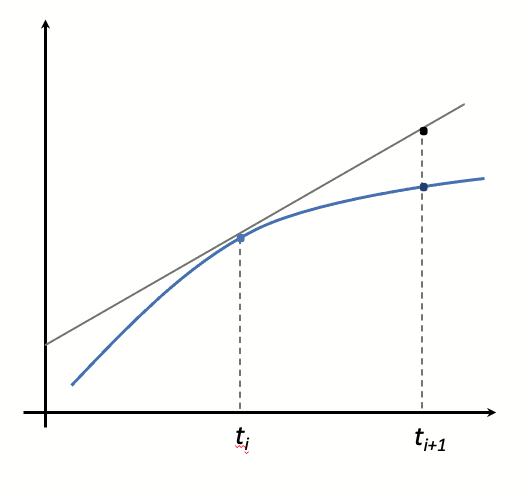
\includegraphics{./figs/euler_time.png}}
  \end{center}
  \caption[]{Euler method}
  \label{fig:euler-time}
\end{figure}

\section{Middle point method}

\begin{figure}
  \begin{center}
    \resizebox{\textwidth}{!}{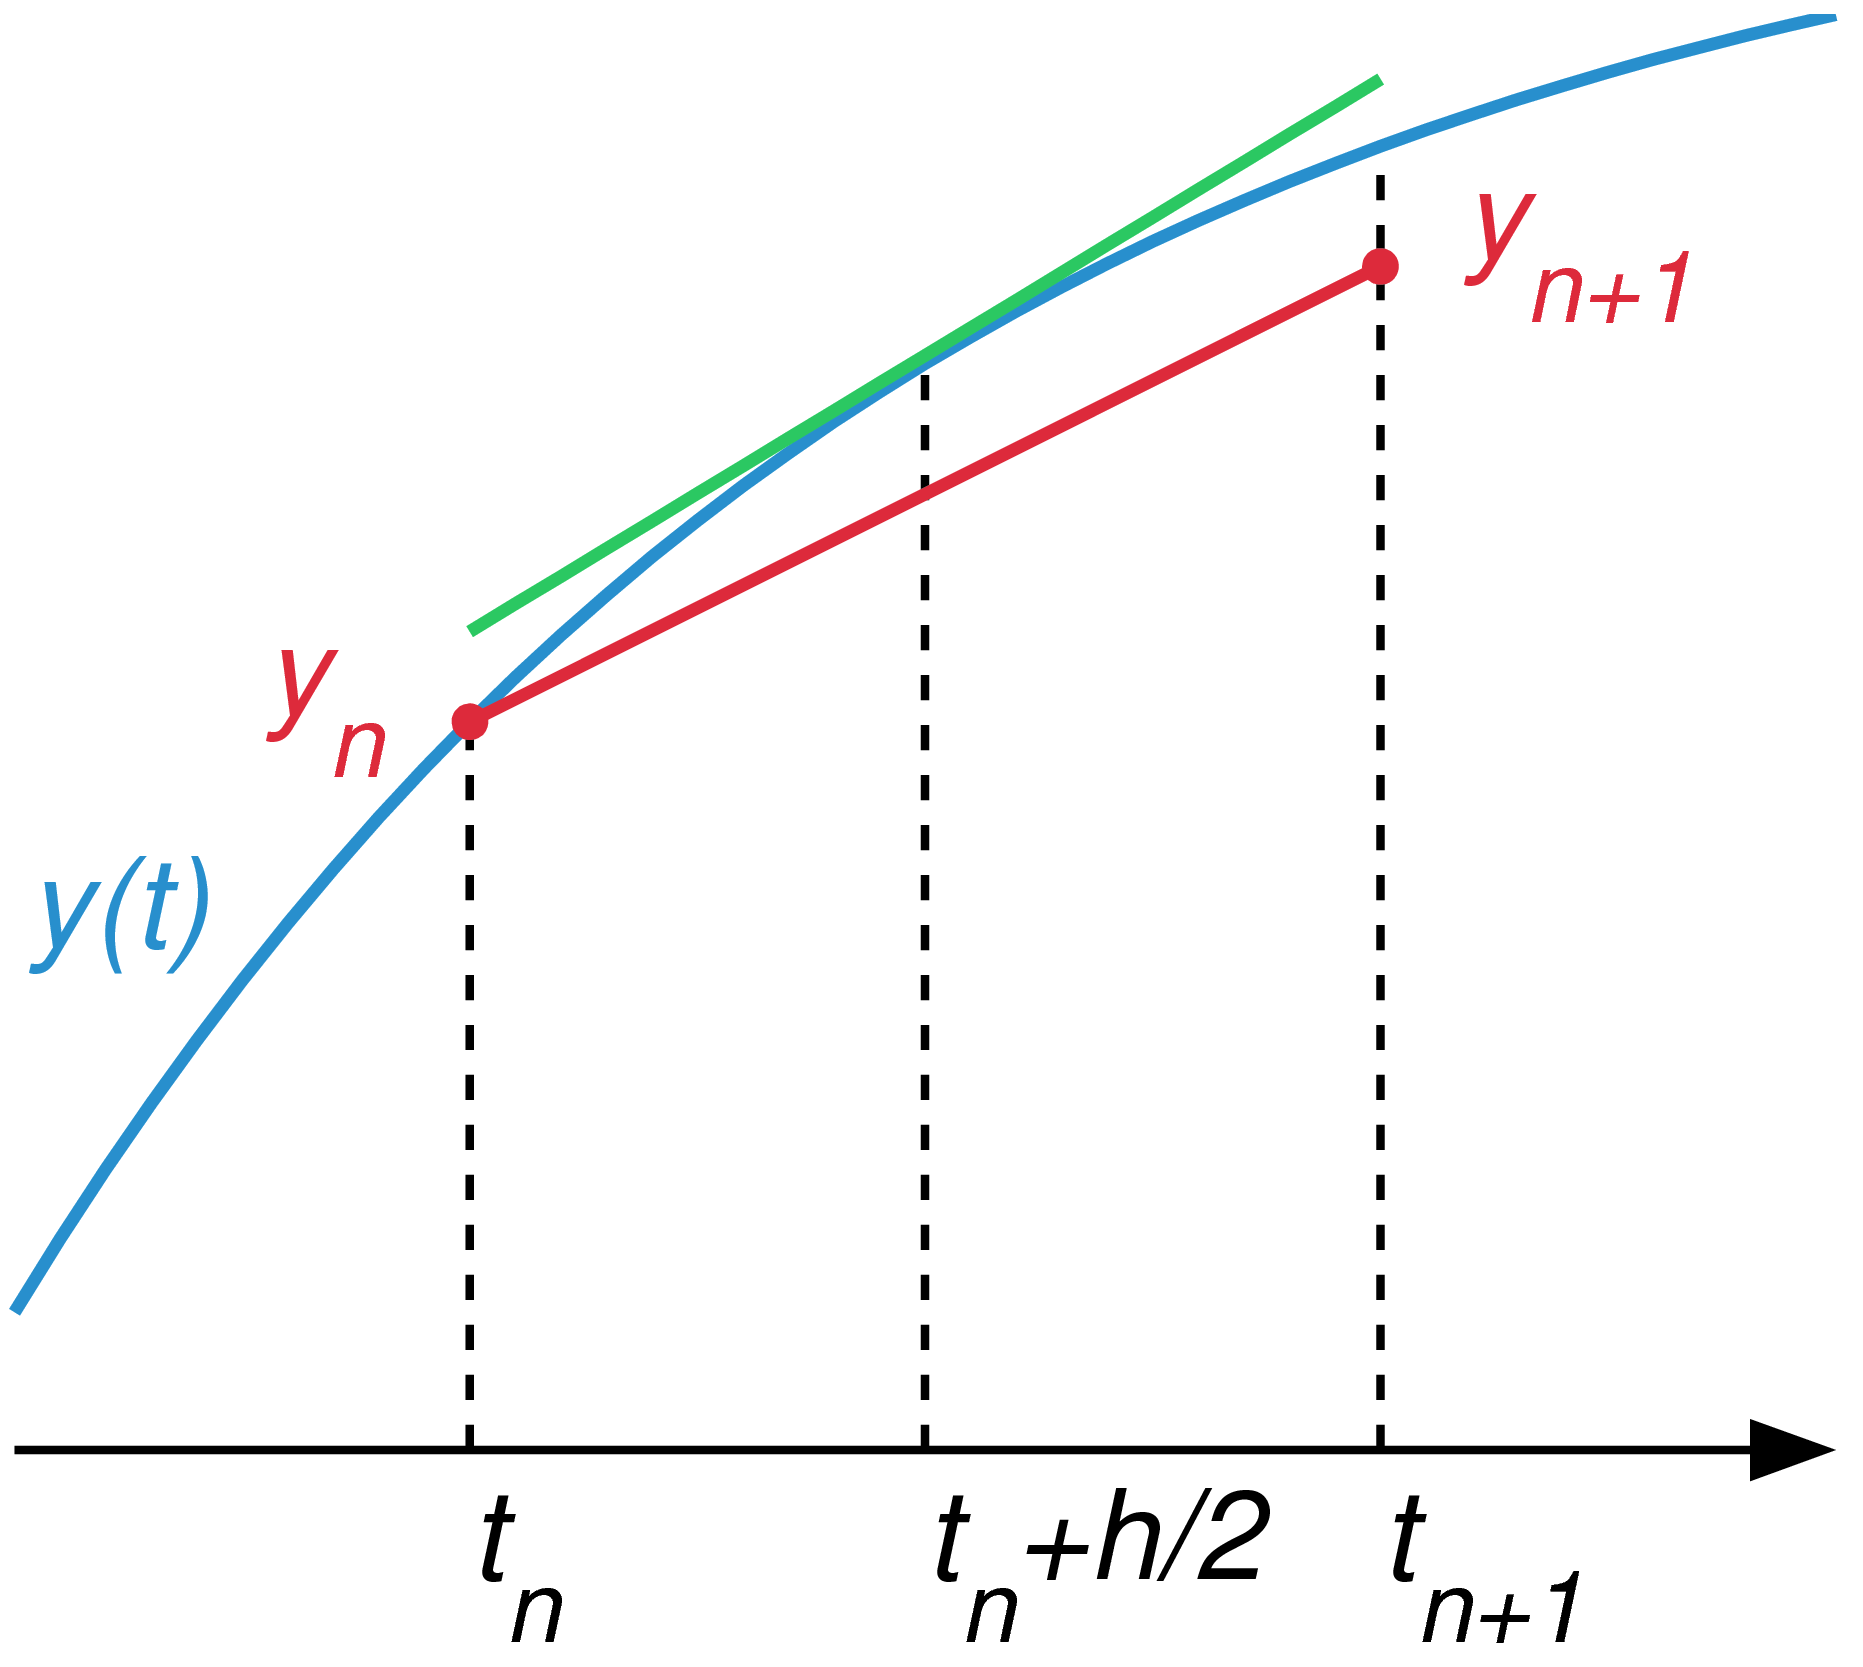
\includegraphics{./figs/Midpoint_method_illustration.png}}
  \end{center}
  \caption[]{Midpoint method}
  \label{fig:midpoint-method}
\end{figure}

Another possibility is to use the slope of the derivative at the midpoint between present and future \figp{fig:midpoint-method}

\beq
\bar{f} = f(t_\nhalf,y_\nhalf)
\eeq

\noindent where $y_\nhalf =y(t+\Delta t/2)$. This is equivalent to the trapezoidal rule for integration 

\beq
\int_t^{t+\Delta t} f(t) dt  \approx \left(\frac{f(t_{n+1}) +  f(t_n)}{2}\right)\Delta t = f(t_\nhalf)\Delta t
\eeq

One can prove that this is equivalent to second order. If $y_\nhalf$
is obtained by the forward Euler integration by half a timestep

\beq
y_\nhalf = y_n + f(t_n,y_n) \frac{\Delta t}{2} 
\eeq

\noindent then

\beqn
y_{n+1} &=& y_n + f(t_\nhalf,y_\nhalf )\Delta t \\
             &=&y_n + f\left(t+\frac{\Delta t}{2},y_n + f(t_n,y_n) \frac{\Delta t}{2} \right) \Delta t \label{eq:xn1}\\
\eeqn

\noindent and because $f(t,y) \equiv d y/d t$,

\beqn
f\left(t+\frac{\Delta t}{2}, y(t) + f(y,t) \frac{\Delta t}{2}\right)&=&\frac{d}{d{\left(t+\frac{\Delta
        t}{2}\right)}} \left(y(t) + f(y,t) \frac{\Delta t}{2}\right)\\
&=&\frac{d y}{d t} + \frac{d f}{d t}\frac{\Delta t}{2}
\eeqn

Substituting into \eq{eq:xn1},

\beq
y_{n+1} = y_n + \frac{d y}{d t}\Delta t +
\frac{d^2 y}{d t^2}\frac{\Delta t^2}{2} +
\mathcal{O}(\Delta t^3)
\eeq

Which shows this approximation has local truncation error of third order. Because it takes $N=T/\Delta t$ timesteps to reach a
solution, the order of the accumulated error is second order. 

\beq
N \ \mathcal{O}(\Delta t^3)  = \mathcal{O}(\Delta t^2)
\eeq

\subsection{Leapfrog}

The leapfrog integration uses the midpoint rule to offset the position and velocities by half a timestep (hence leapfrog). In the system below

\beqn
v_{i+1/2} = v_{i-1/2} + a_i \Delta t \\
x_{i+1} = x_i + v_{i+1/2} \Delta t
\eeqn

where $\ddot{x} = \dot{v} = F(x)$, and $\dot{x}=v$. The
velocities are always calculated at half timesteps, and the positions (and hence accelerations) always at integer timesteps. 

\subsubsection{Order of Leapfrog} 

Applied to a gravitational problem, or any problem where the acceleration depends only on position,
leapfrog in fact achieves 4th order accuracy. Consider $i=0$

\beqn
v_{1/2} = v_{-1/2} + g_0 \Delta t \\
x_1 = x_0 + v_{1/2} \Delta t
\eeqn

and the second derivative $\ddot{x}=g$

\beq
x_1 - 2x_0 + x_{-1} = g_0 \Delta t^2 + \epsilon
\label{eq:leap1}
\eeq

where $\epsilon$ is the truncation error. Expanding in Taylor the points $x_1$ and $x_{-1}$

\beqn
x_1 &=& x_0 + \frac{dx}{dt}\Delta t + \frac{d^2x}{dt^2}\frac{\Delta t^2}{2} + \frac{d^3x}{dt^3}\frac{\Delta t^3}{3!} + \mathcal{O}\left(\Delta t^4\right)\\
x_{-1} &=& x_0 - \frac{dx}{dt}\Delta t + \frac{d^2x}{dt^2}\frac{\Delta t^2}{2} - \frac{d^3x}{dt^3}\frac{\Delta t^3}{3!} + \mathcal{O}\left(\Delta t^4\right)\\
\eeqn

Summing them

\beq
x_1 + x_{-1} = 2x_0 + \frac{d^2x}{dt^2}\Delta t^2 + \mathcal{O}\left(\Delta t^4\right)
\label{eq:leap2}
\eeq

comparing \eq{eq:leap1} and \eq{eq:leap2}, the truncation error is $\mathcal{O}\left(\Delta t^4\right)$

\subsection{Kick-drift-kick}

The kick-drift-kick algorithm uses a version of leapfrog, taking first a half time step in velocity (kick)

\beq
v_{i+1/2} = v_i + a_i\frac{\Delta t}{2}
\label{eq:kick1}
\eeq

\noindent then using that velocity to advance the position (drift)


\beq
x_{i+1} = x_i + v_{i+1/2} \Delta t 
\label{eq:drift}
\eeq

\noindent and finally bringing the velocity to $i+1$ with another half-time step kick, now with acceleration computed in the future

\beq
v_{i+1} = v_{i+1/2} + a_{i+1}\frac{\Delta t}{2}
\label{eq:kick2}
\eeq


The kick-drift-algorithm is this series of steps. Notice between \eq{eq:drift} and \eq{eq:kick2}, the acceleration is computed at point $i+1$. The 1st kick is an Euler step, the drift is a midpoint, and the last kick is an modified Euler, using the derivative at the future point. 

\subsubsection{Time reversibility}

The KDK algorith is time reversible. Notice that if you want to take the backsteps, starting from the second kick and setting $\Delta t \rightarrow -\Delta t$

\beq
v_{i+1/2} = v_{i+1} - a_{i+1}\frac{\Delta t}{2}
\eeq

\noindent all variables are present. Now the drift back in time

\beq
x_{i}= x_{i+1} -	v_{i+1/2} \Delta t
\eeq

\noindent again all variables are present. Finally the last kick back in time

\beq
v_{i} = v_{i+1/2} - a_{i}\frac{\Delta t}{2}
\eeq

\noindent both $x_i$ and $v_i$ are now back at the same spot. 


Trying that with the Euler step does not work. Time-reversing Euler will lead to

\beq
x_i = x_{i+1} - v_i \Delta t
\eeq

\noindent needs $v_i$. One would instead do 

\beq
x_i = x_{i+1} - v_{i+1} \Delta t
\eeq

\noindent which is not the same operation. Similarly with the velocities, the reverse Euler timestep should be

\beq
v_i = v_{i+1} - a_i \Delta t
\eeq

\noindent but instead we would do 

\beq
v_i = v_{i+1} - a_{i+1} \Delta t
\eeq

\noindent which is again not the same operation. 

The time reversibility of KDK leads to the property that the energy error is bound. As such, it is a powerful method for gravitational problems (although there is phase error). 

\section{4th order Runge Kutta}

The Euler method is equivalent to a shooting method, whereas the midpoint rule is equivalent to the trapezoidal rule. A better method would be the equivalent to the Simpson integration rule. This is the 4th order Runge-Kutta, which is the standard for numerical integration

\beq
x(t+\Delta t) = x(t) + \frac{1}{6}\left[f(x_1,t_1) + 2f(x_2,t_2) + 2f(x_3,t_3) +  f(x_4,t_4)   \right]\Delta t
\eeq

It advances by using 4 points in space (beginning end and two intermmediate) and three in time (beginning, middle point, and end)

\beqn
x_1 = x(t) &\quad& t_1 = t\\
x_2 = x(t) + \frac{1}{2}f(x_1,t_1)\Delta t &\quad& t_2 = t+\frac{1}{2}\Delta t\\
x_3 = x(t) + \frac{1}{2}f(x_2,t_2)\Delta t &\quad& t_3 = t+\frac{1}{2}\Delta t\\
x_4 = x(t) + f(x_3,t_3)\Delta t &\quad& t_4 = t+\Delta t\\
\eeqn

The Simpson integration equivalency is evidenced if $f$ does not depend on $x$

\beq
x(t+\Delta t) = x(t) + \frac{1}{6}\left[f(t_1) + 2f(t_2) + 2f(t_3) +  f(t_4)\right]\Delta t
\eeq

and since $t_2=t_3=t_m$

\beq
x(t+\Delta t) = x(t) + \frac{1}{6}\left[f(t_1) + 4f(t_m) + f(t_4)\right]\Delta t
\eeq

which is the Simpson rule

\beq
\int_a^b x(t) dx \approx  \frac{b-a}{6}\left[f(a) + 4f(\frac{a+b}{2}) + f(b)\right]
\eeq


\section{Runge-Kutta methods}

Both the Euler method and the middle-point method are examples of a
larger family of algorithms known as Runge-Kutta methods. The general method
considers \eq{eq:evolution}, \eq{eq:function}, and \eq{eq:bar}


\beqn
y(t+\Delta t ) &=& y(t) + \int_t^{t+\Delta t} f(y^\prime,t^\prime) \ dt^\prime \nonumber\\
f(y,t) &\equiv& \frac{dy}{dt} \nonumber\\
\bar{f} &\equiv& \frac{1}{\Delta t}\int_t^{t+\Delta t} f(y^\prime,t^\prime) \ dt^\prime \nonumber
\eeqn

\noindent and generalizes the solution by approximating the integral
as a weighted sum of points along the way from $t$ to $t+\Delta t$

\beq
\bar{f} \approx \sum_{i=1}^N b_i  k_i
\label{eq:barf}
\eeq


\noindent where

\beq
k_i = f \left(t_n+ c_i \Delta t ,  y_n + \Delta t \sum_{j=1}^{i-1} a_{ij} k_j \right) 
\eeq

%\noindent the points where the function is sampled are 

%\beqn
%t_i \equiv 
%\eeqn

These coefficients are arranged in a so-called {\it Butcher tableau}

\[
\begin{array}
{c|ccccc}
0\\
c_2 & a_{21}\\
c_3 &a_{31} &a_{32} \\
\vdots & \vdots & &\ddots \\ 
c_s& a_{s1}& a_{s2}& \cdots &a_{s,s-1}\\
\hline
& b_1 &b_2 &\cdots &b_{s-1} & b_s 
\end{array}
\]

The numbers along the left side are the coefficients of $\Delta t$ in
the first argument of $f$. The numbers along the bottom are the
coefficients of the $k$s in the expression for the value of $y$ at the
next step. The numbers in the middle of the array are the coefficients
of the $k$s in second argument  of $f$.


%The 4th order Runge-Kutta has tableau

%\[
%  \renewcommand\arraystretch{1.2}
%\begin{array}
%{c|cccc}
%0\\
%\frac{1}{2} & \frac{1}{2}\\
%\frac{1}{2} &0 &\frac{1}{2} \\
%1& 0& 0& 1\\
%\hline
%& \frac{1}{6} &\frac{1}{3} &\frac{1}{3} &\frac{1}{6} 
%\end{array}
%\]


%In general, the main difficulty of the method is to calculate 

%\beqn
%x_i &\equiv& x(t+\alpha_i\Delta t) \\
% &=& x + \beta_{i-1} k_{i-1} 
%\eeqn

The methods differ in

\begin{itemize}
\item the number of terms $N$ in the summation (the order of the method);
\item the position $c_i$ of the nodes where the function is sampled,  and; 
\item the weights $b_i$ give to each node;
\end{itemize}


We can immediately see that for the Euler method, $N=1$, $b_1 =1$ and
$c_1 = 0$, making it a Runge-Kutta method of 1st order. The Butcher tableau for the
Euler method is

\[
    \renewcommand\arraystretch{1.2}
\begin{array}
{c|c}
0 &  \\
\hline
  & 1
\end{array}
\]


The middle point method is also a Runge-Kutta, with $N=2$, with $b_1 = b_2 =
1/2$, $c_1 = 0$ and $c_2 = 1$. These choices give the middle point

\beq
f(x_{1/2},t_{1/2}) = \frac{1}{2}\left(f(x_1,t_1) + f(x_2,t_2)\right)
\eeq

with $t_2 = t_1 + \Delta t$. The Butcher tableau is

\[
  \renewcommand\arraystretch{1.2}
  \begin{array}
{c|ccccc}
0\\
1& 1\\
\hline
  & \frac{1}{2} &\frac{1}{2}
\end{array}
\]

Let us prove this rigorously, in a way that will also lay out the
general method, which will be used for higher order Runge-Kutta
methods. 

\subsection{General method}

The solution for the 2nd order method uses $N=2$, thus

\beq
y_{n+1} = y_n + \Delta t  \left( b_1 k_1 + b_2 k_2\right)
\label{eq:expand}
\eeq

We first choose $c_1 = 0$, defining

\beq
k_1 \equiv f(t_1,y_1) 
\eeq

\noindent which we know since $t_1=t_n$ and $y_1=y_n$ are the initial conditions. We then use this to find $k_2$

\beq
k_2 \equiv f(t_n+c_2 \Delta t,y_n+\Delta t \ a_{21} \ k_1) 
\eeq


\noindent To find $c_2$, $b_1$, $b_2$ and $a_{21}$, we expand $y(t)$ in Taylor series.

\beq
y(t+\Delta t) = y(t) + \frac{d y}{d t}\Delta t +
\frac{d^2 y}{d t^2}\frac{\Delta t^2}{2} +
\mathcal{O}(\Delta t^3) 
\label{eq:taylor}
\eeq

To make the two expressions, \eq{eq:expand} and \eq{eq:taylor} match, we need

\beq
\frac{d y}{d t}\Delta t +\frac{d^2 y}{d
  t^2}\frac{\Delta t^2}{2}  = \Delta t \left(b_1 k_1 + b_2 k_2 \right)
\eeq

substituting $k_1 = f(t_1,y_1) $ and $k_2 =  f(t_2,y_2)$,

\beq
\frac{d y}{d t}\Delta t +\frac{d^2 y}{d t^2}\frac{\Delta t^2}{2}  = b_1 \Delta t f(t_1,y_1) + b_2 \Delta t
f(t_2,y_2)
\eeq

and since $f=\frac{d y}{d t}$, then the second derivative is 

\beqn
\frac{d^2 y}{d  t^2} &=& \frac{d f}{d t}  \\
 &=& \frac{\partial f}{\partial t}  + \frac{\partial y}{\partial t}\frac{\partial f}{\partial  y}\\
  &=& \frac{\partial f}{\partial t}  + f \frac{\partial f}{\partial y}
\eeqn

Substituting the second derivative on the LHS 

\beq
f\Delta t + \left(\frac{\partial f}{\partial t}  + f \frac{\partial f}{\partial y}\right)\frac{\Delta t^2}{2}  = b_1 \Delta t f(t_1,y_1) + b_2 \Delta t
f(t_2,y_2)
\label{eq:mu}
\eeq

now use the multi-variable Taylor expansion for $f(t_2,y_2)$

\beq
f(x_0+\Delta x,y_0+\Delta y) = f(x_0,y_0) + \Delta x \frac{\partial  f}{\partial x} +\Delta y \frac{\partial  f}{\partial y} + \mathcal{O}(\Delta^2) 
\eeq

so that

\beqn
f(t_2,y_2) &=& f(t_1+c_2\Delta t,y_1+\Delta t \ a_{21} \ k_1)\\
&\approx&  f(t_1,y_1) +  c_2\Delta t \frac{\partial  f}{\partial t} + \Delta t \ a_{21} k_1 \frac{\partial  f}{\partial y} 
\eeqn


substituting into \eq{eq:mu}


\beqn
f\Delta t + \left(\frac{\partial f}{\partial t}  + f \frac{\partial f}{\partial y}\right)\frac{\Delta t^2}{2}  &=& b_1\Delta t f + b_2\Delta t \left(f +  c_2\Delta t \frac{\partial  f}{\partial t} + \Delta t \ a_{21} k_1 \frac{\partial  f}{\partial y} \right)\\
&=&(b_1+b_2)\Delta t f + \left(b_2 c_2 \frac{\partial
    f}{\partial t} + b_2 \ a_{21} f \frac{\partial
    f}{\partial y} \right)\Delta t^2
\eeqn

where we also substituted $k_1=f$. These expressions are equivalent if 

\beqn
b_1 + b_2 &=& 1 \\
b_2 \ c_2 &=& \frac{1}{2}\\
b_2 \ a_{21} &=& \frac{1}{2} 
\eeqn

Notice that the
solution is not unique, because these are three equations and four
variables. The choice for the second order Runge-Kutta using middle point is 
$b_1=b_2 = 1/2$, $c_2=a_{21}=1$.  

\section{Runge-Kutta 3rd order}

The solution for the 3rd order method uses $N=3$, thus

\beq
y_{n+1} = y_n + \Delta t  \left( b_1 k_1 + b_2 k_2 + b_3 k_3\right)
\label{eq:expand}
\eeq

with

\beqn
k_1 &=& f(t_1,y_1)\\
k_2 &=& f(t_1 + c_2\Delta t,y_1+\Delta t a_{21} k_1)\\
k_3 &=& f(t_1 + c_3\Delta t,y_1+\Delta t \left(a_{31} k_1+a_{32} k_2\right)) 
\eeqn

\noindent Again, to find the coefficients, we expand $y(t)$ in Taylor
series, now to 3rd order

\beq
y(t+\Delta t) = y(t) + \frac{d y}{d t}\Delta t +
\frac{d^2 y}{d t^2}\frac{\Delta t^2}{2} +
\frac{d^3 y}{d t^3}\frac{\Delta t^3}{6} +
\mathcal{O}(\Delta t^4) 
\label{eq:taylor3}
\eeq

To make the two expressions match, we need
 
\beq
\frac{d y}{d t} +\frac{d^2 y}{d t^2}\frac{\Delta t}{2}+\frac{d^3 y}{d t^3}\frac{\Delta t^2}{6}  = b_1 k_1 + b_2 k_2 + b_3 k_3 
\eeq


We replace the operator $d/dt = \partial_t + f \partial_y$, leading to 

\beqn
\frac{d y}{d t} &=& \left(\partial_t + f \partial_y  \right) y\\
&=& f 
\eeqn

\beqn
\frac{d^2 y}{d t^2} &=& \left(\partial_t + f \partial_y  \right) f \\
&=&f_t + f f_y 
\eeqn

\beqn
\frac{d^3 y}{d t^3} &=& \left(\partial_t + f \partial_y  \right) \left(f_t + f f_y \right)\\
&=& f_{tt} + 2f f_{yt} + f_tf_y + ff_y^2 + f^2 f_{yy} 
\eeqn

now use the multi-variable Taylor expansion for $f(t_2,y_2)$ to 3rd
order 

\beq
f(x_0+\Delta x,y_0+\Delta y) = f(x_0,y_0) + \Delta x f_x +\Delta y f_y + \frac{1}{2}\Delta x^2 f_{xx} +\frac{1}{2}\Delta y^2 f_{yy} + \Delta x\Delta y f_{xy} + \mathcal{O}(\Delta^3) 
\eeq

so we have the expressions for $k_2$ and $k_3$

\beq
k_2 = f + c_2\Delta t f_t + \Delta t a_{21} f f_y + \frac{1}{2}f_{tt}c_2^2 \Delta t^2 + \frac{1}{2}f^2f_{yy}a_{21}^2\Delta t^2+ff_{yt}c_2\Delta t^2 a_{21}
\eeq

\beq
k_3 = f + c_3\Delta t f_t + \Delta t \left(a_{31} f + a_{32}k_2 \right) f_y + \frac{1}{2}f_{tt}c_3^2 \Delta t^2 + \frac{1}{2}f^2f_{yy}\left(a_{31} f + a_{32}k_2\right)^2\Delta t^2+ff_{yt}c_3\Delta t^2 \left(a_{31} f + a_{32}k_2 \right)
\eeq

Substituting $dy/dt$, $d^2y/dt^2$, $d^3y/dt^3$ on the LHS, and $k_2$ and
$k_3$ on the RHS 

\beqn
f + \left(f_t + f f_y\right)\frac{\Delta t}{2} + \left(f_{tt} + 2f f_{yt} + f_tf_y + ff_y^2 + f^2 f_{yy} \right) \frac{\Delta t^2}{6}&=& \nonumber \\
%
b_1 f &+&\nonumber\\
b_2 \left(f + c_2 \Delta t f_t + \Delta t a_{21} f f_y + f_{tt} c_2^2\frac{\Delta t^2}{2} + f^2 f_{yy}a_{21}^2 \frac{\Delta t^2}{2} + ff_{yt}c_2 a_{21}\Delta t^2\right) &+& \nonumber \\
b_3 \left[f + c_3 \Delta t f_t + \Delta t  \left(a_{31} f + a_{32}k_2 \right) f_y + f_{tt} c_3^2\frac{\Delta t^2}{2} + f_{yy}\left(a_{31} f + a_{32}k_2 \right)^2 \frac{\Delta t^2}{2} + ff_{yt}c_3 \left(a_{31} f + a_{32}k_2 \right)\Delta t^2\right]&&\nonumber\\
\eeqn

Expanding now the terms with $k_2$ keeping only the terms up to
$\Delta t^2$,

\beqn
f + \left(f_t + f f_y\right)\frac{\Delta t}{2} + \left(f_{tt} + 2f f_{yt} + f_tf_y + ff_y^2 + f^2 f_{yy} \right) \frac{\Delta t^2}{6}&=& \nonumber \\
%
b_1 f &+&\nonumber\\
b_2 \left(f + c_2 \Delta t f_t + \Delta t a_{21} f f_y + f_{tt} c_2^2\frac{\Delta t^2}{2} + f^2 f_{yy}a_{21}^2 \frac{\Delta t^2}{2} + ff_{yt}c_2 a_{21}\Delta t^2\right) &+& \nonumber \\
b_3 \left(f + c_3 \Delta t f_t + \Delta t  a_{31} f f_y + f_{tt}  c_3^2\frac{\Delta t^2}{2} + f^2 f_{yy}a_{31}^2 \frac{\Delta t^2}{2} +  ff_{yt}c_3 a_{31}  \Delta t^2 + \right.&&\nonumber\\
\left. f\Delta t^2 f_{yt}c_3 a_{32}+\Delta t^2  a_{31}a_{32}f^2f_{yy}+f^2 \frac{\Delta t^2}{2}a_{32}^2f_{yy}+\Delta t a_{32}f_y f + \Delta t^2 a_{32}f_yf_t c_2 + \Delta t^2a_{32}f_y^2fa_{21}\right)&&\nonumber\\
\eeqn

The coefficients that multiply $f$, $f_t$, $ff_y$, $f_{tt}$, $ff_{yt}$, $f_tf_y$, $ff_y^2$,
and $f^2f_{yy}$ lead to the system 

\beqn
b_1 + b_2 + b_3 &=& 1\\
b_2 c_2 + b_3 c_2 &=& \frac{1}{2}\\
b_2 a_{21} + b_3 a_{31} + b_3 a_{32} &=& \frac{1}{2}\\
b_2 c_2^2 + b_3 c_3^2 &=& \frac{1}{3}\\
b_2 c_2 a_{21} + b_3 c_3 a_{31} + b_3 c_3 a_{32} &=& \frac{1}{6}\\
b_3 a_{32} c_2 &=& \frac{1}{6}\\
b_3 a_{32} a_{21} &=& \frac{1}{6}\\
b_2 a_{21}^2 + b_3 a_{31}^2 + 2b_3 a_{31} a_{32} + b_3a_{32}^2 &=& \frac{1}{3}
\eeqn

This system defines the coefficients for 3rd order Runge-Kutta
methods. Kutta's original method was $b_1 = b_3 = 1/6$, $b_2 = 2/3$,
$c_1 = 1/2$, $c_2 = 1$, $a_{21} = 1/2$, $a_{31}=-1$, $a_{32}=2$. The
Butcher tableau is


\[
  \renewcommand\arraystretch{1.2}
  \begin{array}
{c|ccccc}
0\\
\sfrac{1}{2}& \sfrac{1}{2}\\
1& -1 & 2\\
\hline
  & \sfrac{1}{6} &\sfrac{2}{3} & \sfrac{1}{6}
\end{array}
\]

Other 3rd order methods are Heun's


\[
  \renewcommand\arraystretch{1.2}
  \begin{array}
{c|ccccc}
0\\
\sfrac{1}{3}& \sfrac{1}{3}\\
\sfrac{2}{3}& 0 & \sfrac{2}{3}\\
\hline
  & \sfrac{1}{4} &0 & \sfrac{3}{6}
\end{array}
\]

and Ralston's

\[
  \renewcommand\arraystretch{1.2}
  \begin{array}
{c|ccccc}
0\\
\sfrac{1}{2}& \sfrac{1}{2}\\
\sfrac{3}{4}& 0 & \sfrac{3}{4}\\
\hline
  & \sfrac{2}{9} &\sfrac{1}{3} & \sfrac{4}{9}
\end{array}
\]

All these methods are solution to the system. 

\section{Runge-Kutta 4th order}

The 4th order method follows the same procedure. It uses $N=4$, so the summation is 

\beq
y_{n+1} = y_n + \Delta t  \left( b_1 k_1 + b_2 k_2 + b_3 k_3 + b_4k_4\right)
\label{eq:expand}
\eeq

with

\beqn
k_1 &=& f(t_1,y_1)\\
k_2 &=& f(t_1 + c_2\Delta t,y_1+\Delta t a_{21} k_1)\\
k_3 &=& f(t_1 + c_3\Delta t,y_1+\Delta t \left(a_{31} k_1+a_{32} k_2\right)) \\
k_4 &=& f(t_1 + c_4\Delta t,y_1+\Delta t \left(a_{41} k_1+a_{42} k_2+a_{43} k_3\right)) 
\eeqn

\noindent Again, to find the coefficients, we expand $y(t)$ in Taylor
series, now to 4th order

\beq
y(t+\Delta t) = y(t) + \frac{d y}{d t}\Delta t +
\frac{d^2 y}{d t^2}\frac{\Delta t^2}{2} +
\frac{d^3 y}{d t^3}\frac{\Delta t^3}{6} +
\frac{d^4 y}{d t^4}\frac{\Delta t^4}{24} +
\mathcal{O}(\Delta t^5) 
\label{eq:taylor3}
\eeq

To make the two expressions match, we need
 
\beq
\frac{d y}{d t} +\frac{d^2 y}{d t^2}\frac{\Delta t}{2}+\frac{d^3 y}{d t^3}\frac{\Delta t^2}{6}+\frac{d^4 y}{d t^4}\frac{\Delta t^3}{24}  = b_1 k_1 + b_2 k_2 + b_3 k_3 +b_4k_4
\eeq


To get $d^4y/dt^4$, we use  $d/dt= \partial_t + f \partial_y$ on the
expression we found for $d^3y/dt^3$, leading to 

\beqn
\frac{d^4 y}{d t^4} &=& \left(\partial_t + f \partial_y  \right) \left(f_{tt} + 2f f_{yt} + f_tf_y + ff_y^2 + f^2 f_{yy} \right)\\
&=& f_{ttt} + 3f_tf_{yt} + 3ff_{ytt} + f_{tt}f_y + f_tf_y^2 +5ff_yf_{yt} + 3ff_tf_{yy} + 3f^2f_{yyt} + ff_y^3 +4f^2f_yf_{yy} + f^3 f_{yyy}\nonumber\\
\eeqn

now use the multi-variable Taylor expansion for $f(t,y)$ to 3rd order
to define $k_2$, $k_3$, and $k_4$

\beqn
f(x_0+\Delta x,y_0+\Delta y) &=& f(x_0,y_0) \nonumber\\
&+&\Delta x f_x +\Delta y f_y \nonumber\\
&+& \frac{1}{2}\Delta x^2 f_{xx} +\frac{1}{2}\Delta y^2 f_{yy} +\Delta x\Delta y f_{xy}\nonumber\\
&+& \frac{1}{6}\Delta x^3 f_{xxx} +\frac{1}{6}\Delta y^3 f_{yyy} +\frac{1}{2}\Delta x^2\Delta y f_{xxy}+\frac{1}{2}\Delta x\Delta y^2 f_{xyy}\nonumber\\
&+& \mathcal{O}(\Delta^4) 
\eeqn


From now on the algebra is (very) messy and tedious, but
straightforward. The resulting butcher tableau is


\[
  \renewcommand\arraystretch{1.2}
  \begin{array}
{c|cccccc}
0\\
\sfrac{1}{2}& \sfrac{1}{2}\\
\sfrac{1}{2}& 0 & \sfrac{1}{2} & 0 \\
1& 0 & 0 & 1\\    
\hline
  & \sfrac{1}{6} &\sfrac{1}{3} & \sfrac{1}{3} & \sfrac{1}{6}
\end{array}
\]


Notice that the 4th order Runge-Kutta is equivalent to the Simpson
integration rule. The points are

\[
x(t+\Delta t) = x(t) + \frac{1}{6}\left[ f(x_1^\prime,t_1^\prime) +
  2f(x_2^\prime,t_2^\prime) + 2f(x_3^\prime,t_3^\prime) +
  f(x_4^\prime,t_4^\prime)\right]\Delta t
\]

\beqn
x_1^\prime&=& x(t)\\
x_2^\prime&=& x(t)+\frac{1}{2}f(x_1^\prime,t_1^\prime) \Delta t\\
x_3^\prime&=& x(t)+\frac{1}{2}f(x_2^\prime,t_2^\prime) \Delta t\\
x_4^\prime&=& x(t)+f(x_3^\prime,t_3^\prime) \Delta t
\eeqn

and

\beqn
t_1^\prime&=& t\\
t_2^\prime&=& t+\frac{1}{2}\Delta t\\
t_3^\prime&=& t+\frac{1}{2}\Delta t\\
t_4^\prime&=& t+\Delta t
\eeqn

If $f$ does not depend on $x$


\[
x(t+\Delta t) = x(t) + \frac{1}{6}\left[ f(t_1^\prime) +
  4f(t_m^\prime) +
  f(t_4^\prime)\right]\Delta t
\]

where $t_m = t_2 = t_3$ is the middle point. If $h = \Delta t/2$, and
setting $t_1 = t_a$ and $t_4 = t_b$

\[
x(t+\Delta t) = x(t) + \frac{1}{3}\left[ f(t_a^\prime) +
  4f(t_m^\prime) +
  f(t_b^\prime)\right]h
\]

which is Simpson's rule. The 2/2 split comes from considering a
different point in space.

\subsection{Discontinuities}

\subsubsection{Bulk viscosity}

To deal with discontinuties in a high-order non-conservative method,
we borrow a concept from non-ideal gases, which is the notion
of {\it bulk viscosity}, also referred to as volume viscosity, or second
viscosity. It represents the fluid's resistance to
compression, which microphysically stems from the finite
time it takes for energy given to the fluid to be distributed to the
rovibrational molecular modes. Monoatomic gases and ideal gases do not have bulk
viscosity.

Another way to think of second viscosity is the dissipation that
happens while the gas is out of equilibrium following an expansion or
compression event. Usually the restoration of equilibrium is fast, but
if the relaxation time is long, dissipation will occur. 

Its general form in the NS equation is to add a term to the viscous
tensor that is proportional to the flow divergence

\beq
\pi_{ij}=[...] - \rho\zeta \delta_{ij} \Div{\v{u}}
\label{eq:pizeta}
\eeq

With corresponding acceleration 

 \beqn
 f_\nu(u,\rho) &=& -\rho^{-1}\Div{\v{\pi}} \\
 &=&\zeta\left[ \grad{\left(\Div{\v{u}}\right)} + \left(\grad{\ln\rho}+\grad{\ln\zeta}\right) \Div{\v{u}}\right]
\label{eq:zeta-acceleration}
 \eeqn

% But what does it have to do with discontinuities? As it turns out,
% volume viscosity behaves much as we expect dissipation in a shock to behave. In any
% rapid process, the fluid deviates from equilibrium, but quickly
% returns to it. If, however, the time to return to equilibrium is
% long, dissipation can happen during this long expansion or
% compression. 
  
%div(nu_shock*grad(uu_i))

% tmp=nu_shock*(p%shock*(p%divu*p%glnrho+p%graddivu)+p%divu*p%gshock)

Using a bulk viscosity to deal with shocks in numerical schemes was
first proposed by von Neumann \& Richtmyer (1950). The idea is to add
an artificial viscosity that acts on the shortest resolvable length
scale in the grid. This artificial bulk viscosity will simply smooth a
 discontinuity to a width that can be resolved by the stencil \figp{fig:shock-viscosity}. As long
 as the shock viscosity coefficient can be written in the form
 \eq{eq:pizeta} so its divergence is taken to find the acceleration
 \eq{eq:zeta-acceleration}, the term conserves momentum. 

\begin{figure}
  \begin{center}
    \resizebox{\textwidth}{!}{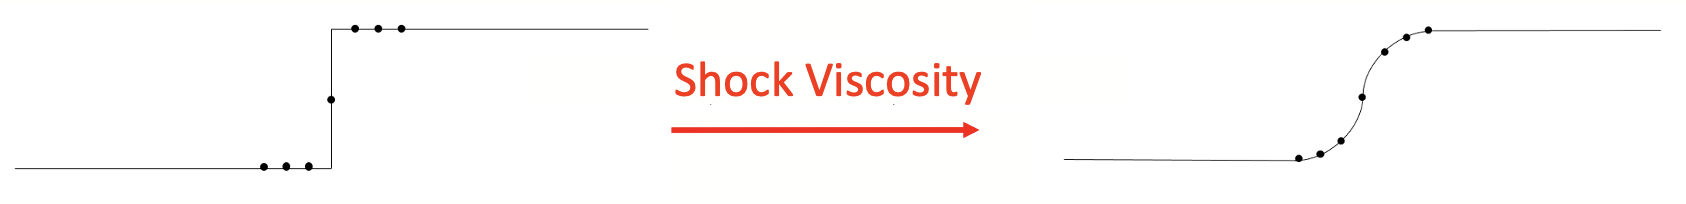
\includegraphics{./figs/shockviscosity.png}}
  \end{center}
  \caption[]{Shock viscosity is used to smooth a discontinuity to the
    point it can be resolved by the stencil.}
  \label{fig:shock-viscosity}
\end{figure}

Consider a constant bulk viscosity coefficient, so that

\beq
\frac{\partial \v{u}}{\partial t} = \zeta\grad{\left(\Div{\v{u}}\right)} 
\eeq

\noindent as is, this is not what we want, since this formulation
operates on both expansion and compression. We want the
force to be zero for expansion ($\Div{\v{u}} > 0$), and activate only for
compression ($\Div{\v{u}}<0$). Thus, the make the $\zeta$ coefficient
proportional to the convergence part only

\beq
\zeta \propto \left(-\Div{\v{u}}\right)_+ 
\eeq

where the $+$ subscript says that only the positive part is
considered. It work as $f(x) = {\rm max}(0, x)$. As such, the
coefficient is

\beq
\zeta \propto \left\{
  \begin{array}{ll}
       -\Div{\v{u}}& {\rm if} \quad -\Div{\v{u}} >0 \\
      0 & {\rm if} \quad -\Div{\v{u}} < 0 \\
\end{array} 
\right.
\eeq

We can define a coefficient of shock viscosity $\nu_{\rm sh}$ to replace the
proportionality. To keep this coefficient close to unity, we will
normalize it by $\Delta x^2$ (since the artificial viscosity operates
on the Laplacian) 


\beq
\boxed{
  \zeta = \nu_{\rm sh}\left(-\Div{\v{u}}\right)_+ \Delta x^2
  }
\eeq

This is the form of the artificial shock viscosity proposed by von
Neumann \& Richtmyer. The acceleration due to shock viscosity is therefore

 \beqn
 f_\nu(u,\rho) &=& -\rho^{-1}\Div{\v{\pi}} \\
 &=&\zeta\left[ \grad{\left(\Div{\v{u}}\right)} + \left(\grad{\ln\rho}+\grad{\ln\zeta}\right) \Div{\v{u}}\right]
 \eeqn

Such a viscosity scheme ensures that energy is dissipated in regions
of the flow where shocks occur, whereas more quiescent regions are
left untouched. Notice that the acceleration is quadratic on the
divergence, so it will be stronger in shock regions than on the smooth
flow. 

The formulation for shock diffusion is similar, yielding

\beq
 f_D(\rho) = \zeta\left(\Laplace{\rho} + \grad{\ln\zeta}\cdot\grad{\rho}\right)
\eeq

This artificial viscosity has the good property that it only becomes
strong when its presence is required, and becomes negligible when the
flow is smooth. It is therefore much better than an uncontrolled
numerical diffusivity. As such, the von Neumann-Richtmyer artificial
viscosity, and varieties thereof, is used in a great many numerical hydrodynamics codes.

A few problems with the scheme are: the viscosity
affects the pre-shock region and the shock is therefore not as sharp
anymore as we had before. Also, it is not sufficient to completely
eliminate post-shock oscillations. Only a linear term can achieve
that, which is Godunov's theorem: 

{\it Linear numerical schemes for solving partial differential equations that do not generate
new extrema (i.e., preserve monotonicity), can be at most first-order accurate.}

%reduces the order of the scheme,
%since at the discontinuity only first order is achieved. 


The high-order schemes presented so far are the ``road less
traveled''.  Some hydrodynamics codes are based on such higher-order
numerical derivatives, like the {\it Pencil Code} that I
develop. Colloquially it is usually said that higher-order
schemes are more accurate than lower-order schemes.
However, this is only true if the function $f(x)$ is reasonably
smooth over length scales of order $\Delta x$.
In other words: the ${\mathcal O}(\Delta x^4)$ is only significantly
smaller than ${\mathcal O}(\Delta x^2)$ if $\partial^5_xf(x)\Delta x^4
\ll \partial^3_xf(x)\Delta x^2 \ll \partial_x f(x)$. That is, if the
higher order derivatives are smaller compared to the lower order
ones: {\it if the function is smooth}.
Higher-order schemes are therefore useful for flows that have no strong
discontinuities in them. This is often true for subsonic flows,
i.e. flows for which the sound speed is much larger than the typical
flow speeds. For problems involving shock waves and other types of
discontinuities such higher-order schemes turn out to be worse than
lower order ones. 

\section{Godunov schemes}

The standard
approach to grid-based astrophysical hydrodynamics is to use the
conservation form of the equations of motion 

\beq
\frac{\partial q}{\partial t} + \Div{f(q)} = 0 
\label{eq:flux-godunov}
\eeq

where here we changed the notation: $q$ for quantity, and $f(q)$ for
flux of the quantity. We will also introduce the concept of {\it cells}. The idea of flux conserving schemes is to create cells out of the grid, instead of just sampling grid
points. The grid points now become cell centers located at $x_i$, and
we now have cell interfaces or cell walls located at the
half-points. In 3D the cells can  be regarded as control volumes
containing our conserved quantities. 

Let us consider the 1D version of \eq{eq:flux-godunov}

\beq
\frac{\partial q}{\partial t} + \frac{\partial f}{\partial x} = 0 
\label{eq:flux-godunov-1D}
\eeq

and integrate it in time and space

\beq
\int_{x_1}^{x_2}\int_{t_1}^{t_2}\frac{\partial q}{\partial t} +
\frac{\partial f}{\partial x} dx dt = 0 
\eeq

bracketing the time evolution of $q$ and space evolution of $f$

\beq
\int_{x_1}^{x_2}\left[\int_{t_1}^{t_2}\frac{\partial q}{\partial t}dt\right]dx +
\int_{t_1}^{t_2}\left[\int_{x_1}^{x_2}\frac{\partial f}{\partial x} dx \right]dt = 0 
\eeq

the bracketed are substituted by the quantities themselves

\beq
\int_{x_1}^{x_2} \left[q(t_2)-q(t_1)\right] dx +
\int_{t_1}^{t_2}\left[f(x_2)-f(x_1) \right]dt = 0 
\eeq


%Let us discretize \eq{eq:flux-godunov}. With an Euler time discretization it yields

%\beq
%\frac{q_i^{n+1}-q_i^{n}}{\Delta t} = -\frac{\left( f_{i+\sfrac{1}{2}}  - f_{i-\sfrac{1}{2}}    \right)}{\Delta x} 
%\eeq

%where
we define the value at point $i$ as the average value of the
quantity integrated over the cell 

\beq
q_i^n = \frac{1}{\Delta x} \int_{x_i-1/2}^{x_i+1/2} q(x,t^n) dx 
\eeq

So we identify $x_1 = x_{i-1/2}$ and $x_2 = x_{i+1/2}$ as cell interfaces.

Similarly, for the time integrals

\beq
f_i^{n+1/2} = \frac{1}{\Delta t} \int_{t^n}^{t^{n+1}} f(x_i,t) dt 
\eeq


%in this form, we can cast the equation as

%\beq
%\int_{x_i-1/2}^{x_i+1/2}\int_{t^n}^{t^{i+1}} \left[\frac{\partial \v{u}}{\partial t} + \frac{\partial\left[F(\v{u})\right]}{\partial x} \right] dx dt = 0  
%\eeq

%so we the fluxes should be computed at the midpoint in time 

we end up with the advection problem in flux-conserving form.

\beq
q_i^{n+1} = q_i^{n}-\frac{\Delta t}{\Delta x} \left[ f^{n+1/2}_{i+\sfrac{1}{2}}  - f^{n+1/2}_{i-\sfrac{1}{2}}    \right]
\label{eq:advect-conserve}
\eeq

%where we define the time-averaged flux function as

%\beq
%F^{n+1/2}_{i+\sfrac{1}{2}} = \frac{1}{\Delta t} \int_{t^n}^{t^{n+1}} F(x_{i+1/2},t) dt 
%\eeq


%\eq{eq:advect-conserve} is the 

%%%% Price's text

%The key insight is to compute the flux at the interface between two
%adjacent cells. The idea of Godunov methods is to compute this flux by
%considering adjoining cells as the left and right states of a
%Riemann problem. In Godunov’s original method, one considers every pair of
%cells to be a shock. This results in a first order scheme by
%virtue of Godunov’s theorem. The way around this 
%is to no longer consider the values $\v{u}$ in the left and right states
%as constant, but instead to use the gradients to reconstruct the
%values of $\v{u}$ at the interface. In smooth flow, the reconstruction
%is exact and no dissipation occurs — because there is no
%jump in the fluid variables to produce irreversible dissipation.
%Reconstruction thus restores higher order convergence of the
%scheme in smooth flow. However, by Godunov’s theorem it is
%impossible to provide second order accuracy at shocks without
%re-introducing post-shock oscillations. So reconstruction is
%done with ``slope-limited'' gradients to ensure that the scheme
%remains monotone (i.e., does not introduce new maxima or
%minima). Slope limiters thus revert to the required first order
%accuracy when the gradients are discontinuous.

%When reconstruction is employed, it is no longer necessary
%to exactly solve the Riemann problem. For many applications
% an approximate solution will suffice, even though approximate
% Riemann solvers are more dissipative than exact solvers.

%% 
 
Since we (by definition of the fact that we solve a numerical problem) do not know exactly what
this average state is, it is the task of the algorithm to provide a recipe that estimates this as well
as possible. In the two examples below we shall describe two such algorithms.
 
 %because, for example, the above assumes that every discontinuity
%is a shock, rather than considering shocks, rarefactions and
%contact discontinuities separately. 

%The simplest ``approximate Riemann solver'' uses the ``local Lax-Friedrichs'' flux
%given by

\subsection{Donor-cell advection}

The simplest flux conserving scheme is the donor-cell scheme. In this scheme the ``average
interface state'' is simply $\tilde{q}_{i+1/2} \approx q_i$, i.e. the value of the
upwind cell. 

\beq
f_{i+1/2}^{n+1/2} \approx q_i^n u_{i+1/2}
\eeq

The physical interpretation of this method is the following. One assumes that the density is
constant within each cell. We then let the material flow through the cell interfaces, from left to
right. Since the density to the left of the cell interface is constant, and since the
CFL condition makes sure that the flow is no further than 1 grid cell spacing at maximum, we
know that for the whole time between time $t_n$ and time $t_{n+1}$,
the flux through the cell interface $\tilde{q}_{i+1/2} ^n u_{i+1/2}
\approx q_i^n u_{i+1/2}$ is constant. Once the time step if finished, the state
in each cell has the form of a step function. To get back to the original sub-grid model
we need to average the quantity $q(x)$ out over each cell, to obtain the new $q^{n+1}_i$ . This is what
happens in the donor-cell algorithm.

Notice that the scheme is very similar to the upwind scheme, in fact
identical if the velocity is constant, yielding the recurrence
relation

\beq
q_i^{n+1} = (1-C)q_i^n  + Cq_{i-1}^n
\eeq

The Donor-Cell algorithm is easily implemented
but, as the upstream differencing method, it is very diffusive.

\subsection{Slopes of the donor cell: Piecewise linear methods}

The donor-cell algorithm is a simple algorithm based on the idea that at the beginning of each
time step the state within each cell is constant throughout the cell. The state at the grid
center is therefore identical to that in the entire cell. The idea that the state is constant in the cell
is, however, just an assumption. One must make some assumption, because evidently we have
not more information about the state in the cell than just the cell-center state. But one could
also make another assumption. One could, for instance, assume that the state within each cell
is a linear function of position. One says that the state is assumed to be piecewise linear. The assumption that it is a linear function within the cell is called a subgrid model: it is
a model of what the state looks like at spatial scales smaller than the grid spacing. The procedure
of creating a subgrid model based on a discrete value at the cell
center is called reconstruction. The piecewise linear scheme we discuss here is therefore a scheme based on piecewise linear
reconstruction of the function from the discrete values. Such a method
also allows for higher order versions (such as the piecewise parabolic reconstruction, seen later). 

The next schemes use the concept of the {\it slope} of the donor cell, where the half-integer fluxes are approximated by 

\begin{equation}
f_{i+1/2} = v\left[ q_{i} + \frac{1}{2}\delta q_i \ \mbox{sign}(v) \ (1-C) \right]
\end{equation}


For positive velocity, this simplifies into 

\begin{equation}
f_{i+1/2} = v\left[ q_{i} + \frac{1}{2}\delta q_i (1-C) \right]
\end{equation}

So it is just the donor cell value $q_{i}$, with a term that depends on the slope of the function over the cell, a quantity still to be defined. The different schemes differ in how they define the slope $\delta q_i$

\subsection{Linear Slopes}

At each grid cell $i$, one can choose between two "natural" slopes to use. These slopes are determined by the difference between the points $i$ and $i+1$ (forward slope) and that between the points $i-1$ and $i$ (backward slope).  


\subsection{Lax-Wendroff}

The Lax-Wendroff scheme uses the forward slope

\begin{equation}
\delta q_i = \delta q_{\rm forward} = q_{i+1} - q_i
\end{equation}


\begin{figure}
  \begin{center}
    \resizebox{\textwidth}{!}{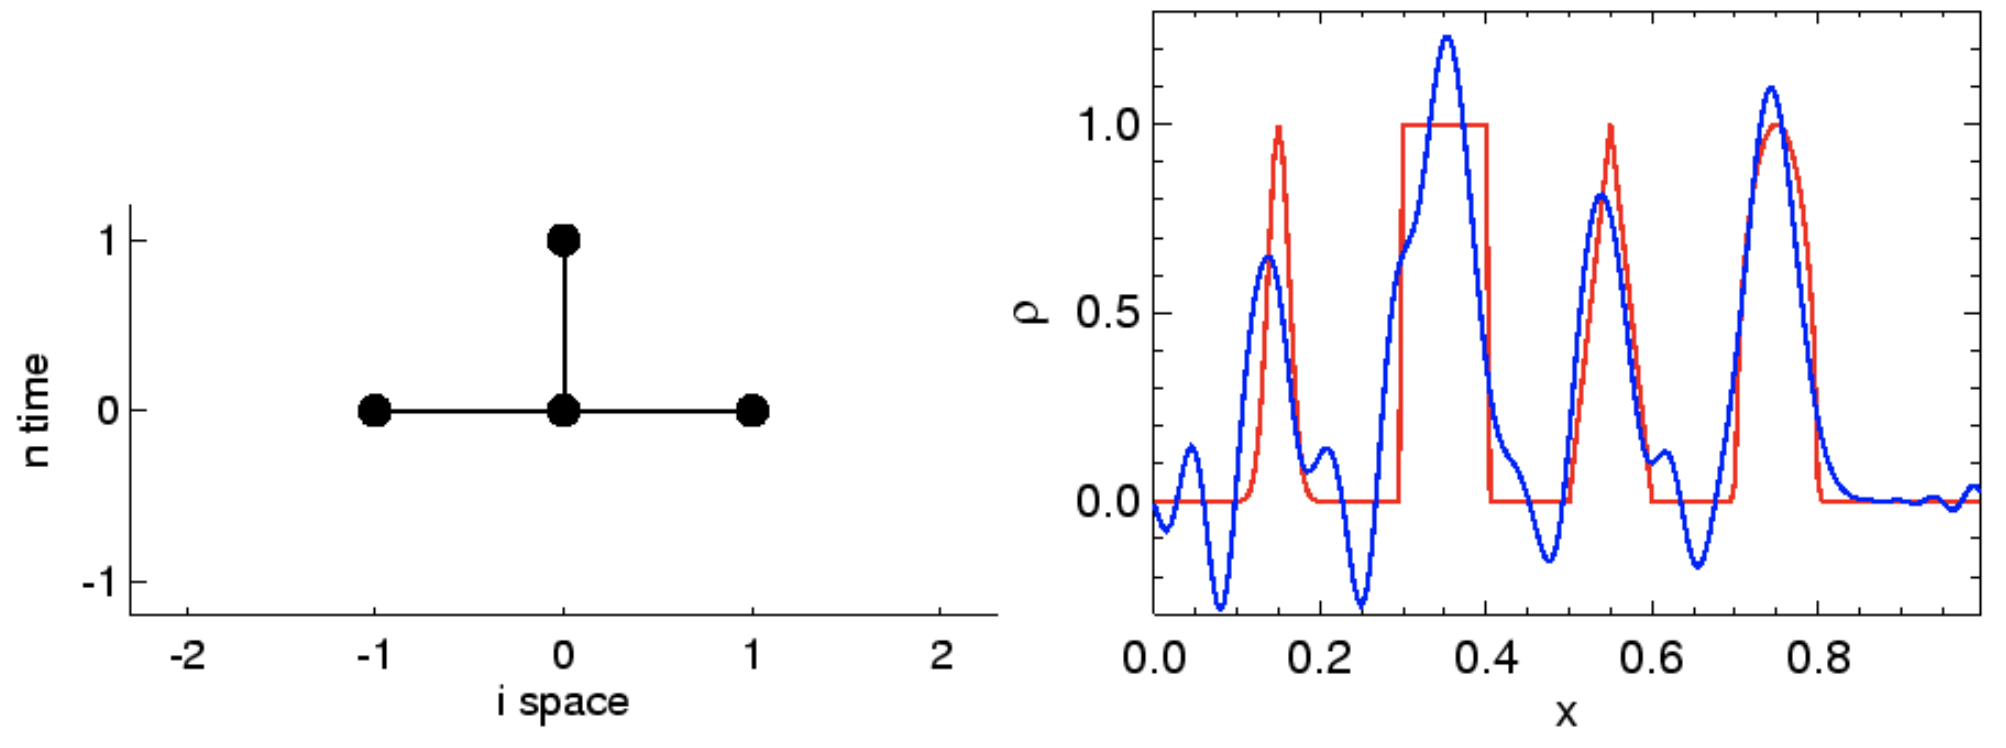
\includegraphics{./figs/laxwendroff.png}}
  \end{center}
  \caption[]{Lax-Wendroff}
  \label{fig:lax-wendroff}
\end{figure}

The result is smooth \figp{fig:lax-wendroff} with considerable overshoot (that, however, does not grow in time). This scheme might be useful for more regular initial conditions.

\subsection{Beam-Warming}

The Beam-Warming scheme \figp{fig:beam-warming} uses the backward slope

\begin{equation}
\delta q_i = \delta q_{\rm backward} = q_{i} - q_{i-1}
\end{equation}

\begin{figure}
  \begin{center}
    \resizebox{\textwidth}{!}{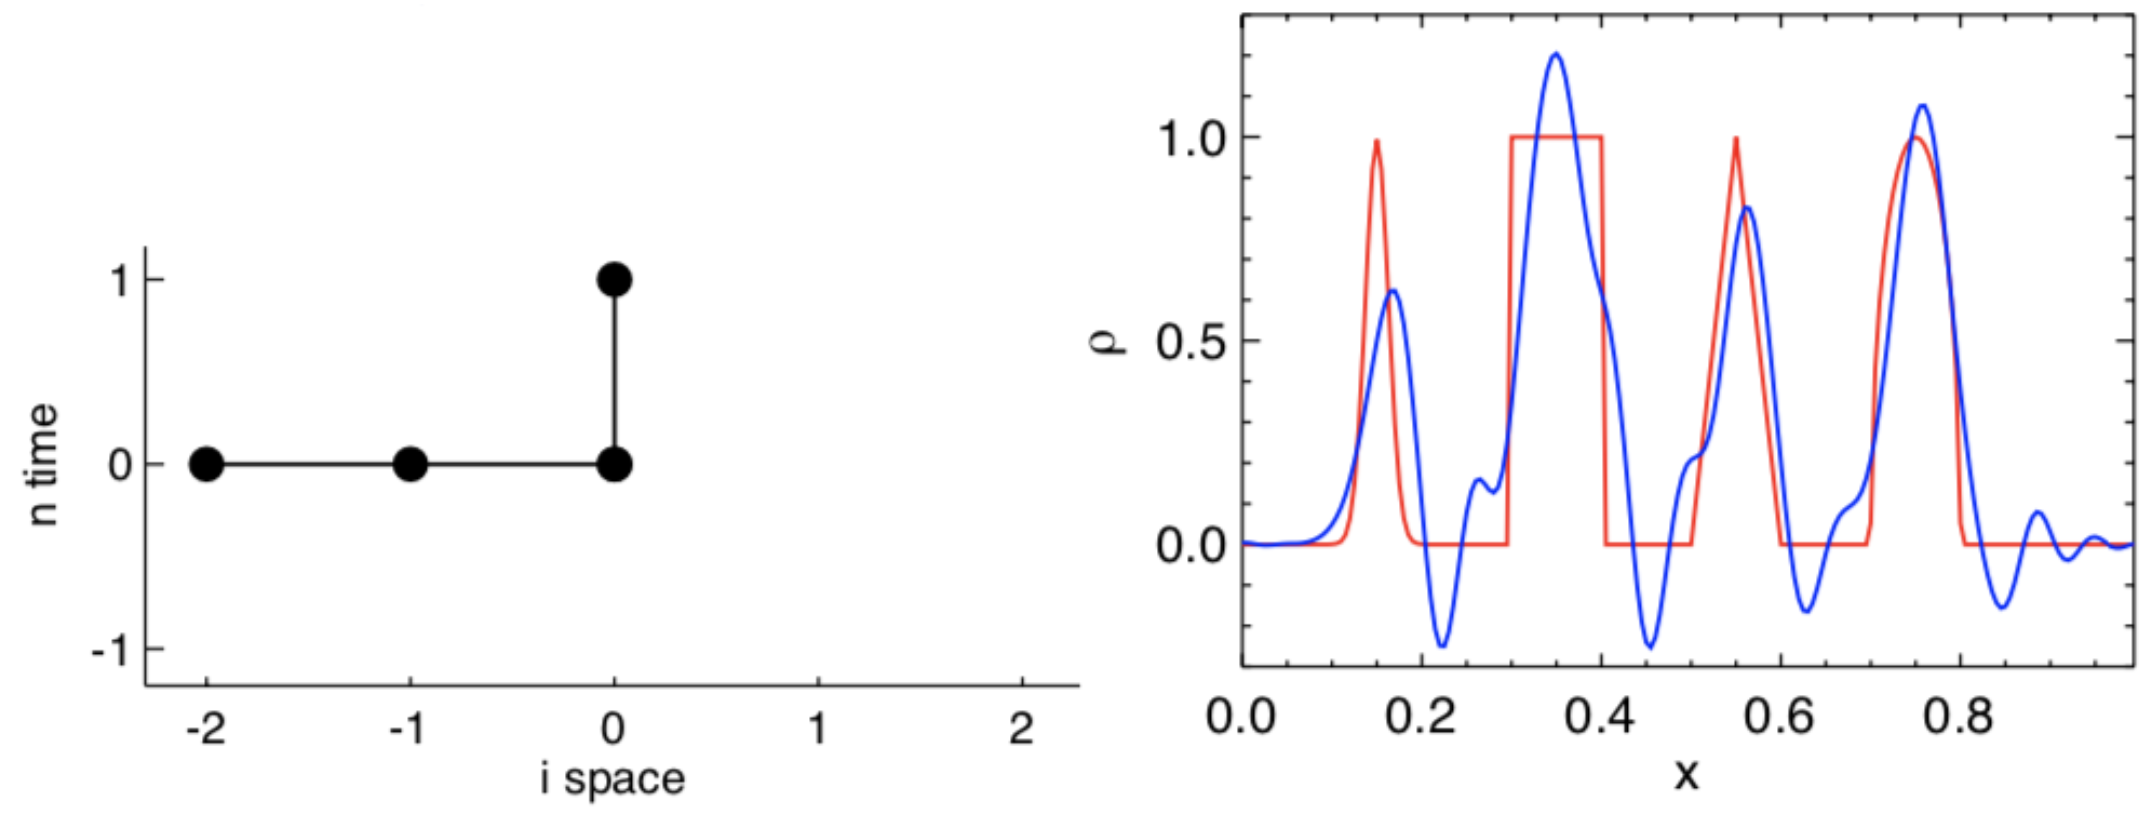
\includegraphics{./figs/beam-warming.png}}
  \end{center}
  \caption[]{Beam-Warming}
  \label{fig:beam-warming}
\end{figure}

\subsection{Fromm}

The Fromm scheme is the average of forward and backward

\begin{equation}
\delta q_i = \frac{1}{2}\left(\delta q_{\rm forward}+\delta q_{\rm backward}\right)
\end{equation}

\begin{figure}
  \begin{center}
    \resizebox{\textwidth}{!}{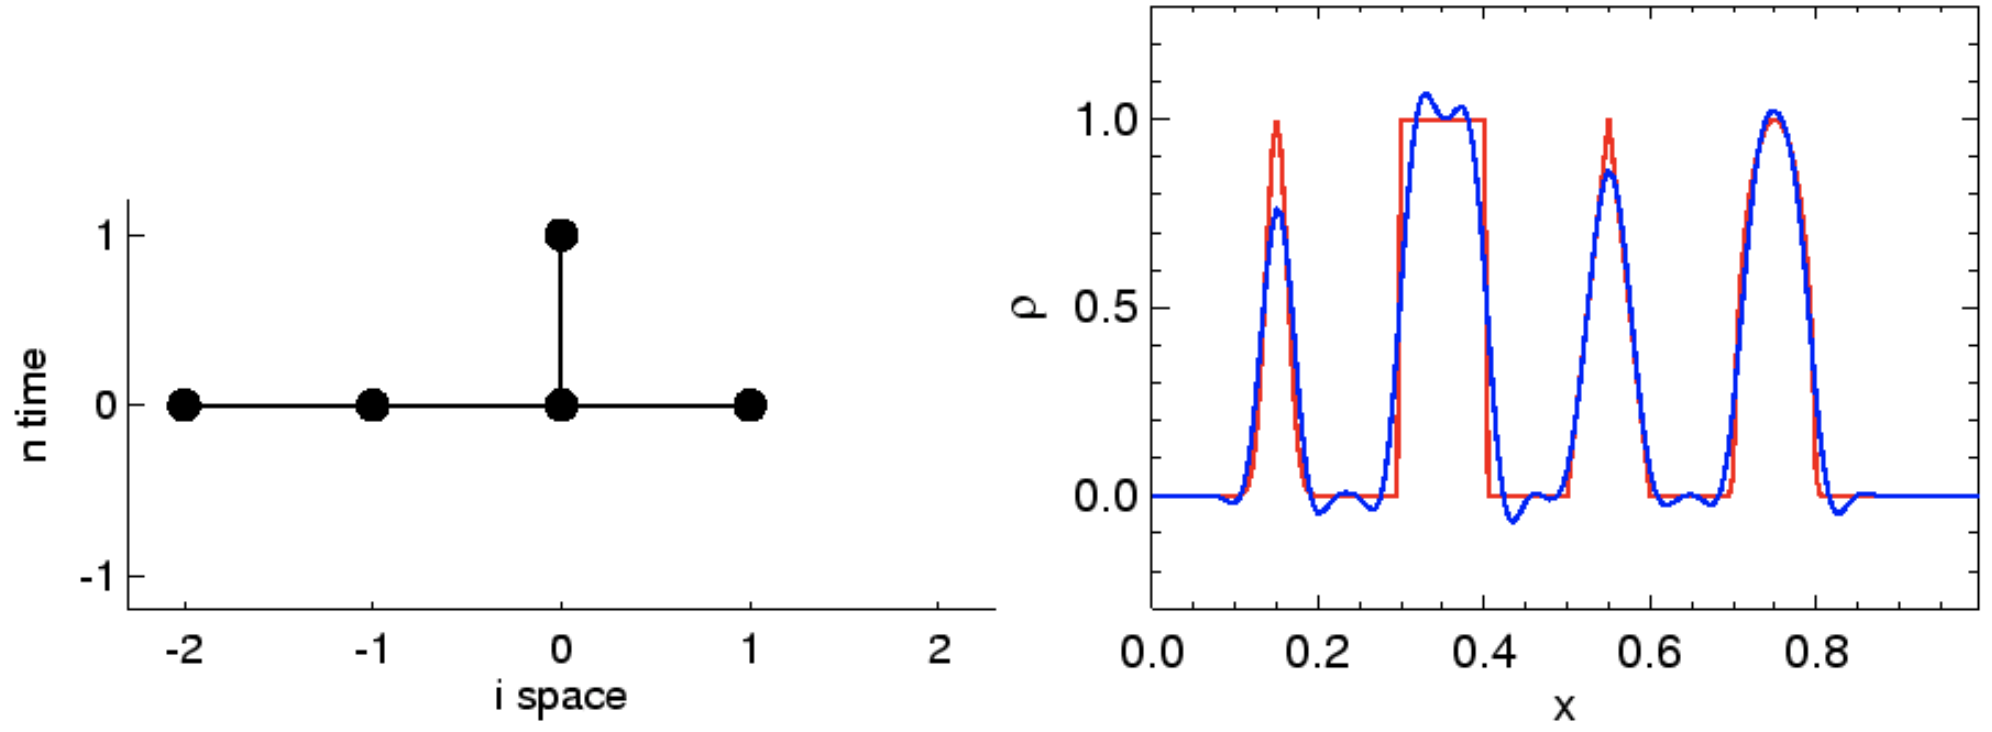
\includegraphics{./figs/fromm.png}}
  \end{center}
  \caption[]{Fromm}
  \label{fig:fromm}
\end{figure}

The result is smooth with some amount of overshoot \figp{fig:fromm}. The initial shape
of the spikes is recognizable. So far the best scheme, if the
overshoot can be accepted.

\subsection{Nonlinear Slopes}

The nonlinear schemes are also called {\bf slope limiters}. They are
non-linear tools to prevent overshoots. With the current piecewise linear geometric picture of the higher
order methods we can gain a geometrical understanding of why such an overshoot occurs. 

In this picture the overshoot happens because the piecewise linear elements can have overshoots. A succesful method to prevent such overshoots is the use of slope limiters. These are
non-linear conditions that modify the slope if, and only if, this is necessary to prevent overshoots. This means that, if this is applied to for instance the Lax-Wendroff method, the slope
limiter keeps the higher (2nd) order nature of the Lax-Wendroff method in regions of smooth variation
of $q$ while it will intervene whenever an overshoot threatens to take place.

In these
schemes, nonlinear corrections are inserted with the purpose of
hindering the oscillations from going unstable. The way these schemes
achieve this result is by limiting the slope to well-behaved
values. We will try three slope limiters: MinMod, Van Leer, and
Superbee.

\subsubsection{MinMod}

In the MinMod slope limiter, the slope is determined by 

\begin{eqnarray}
\delta q_i &=& \mathrm{min}[\mathrm{max} (\delta q_f,0),\mathrm{max}(\delta q_b,0)] \\
&+& \mathrm{max}[\mathrm{min} (\delta q_f,0),\mathrm{min}(\delta q_b,0)]
\end{eqnarray}

\begin{figure}
  \begin{center}
    \resizebox{\textwidth}{!}{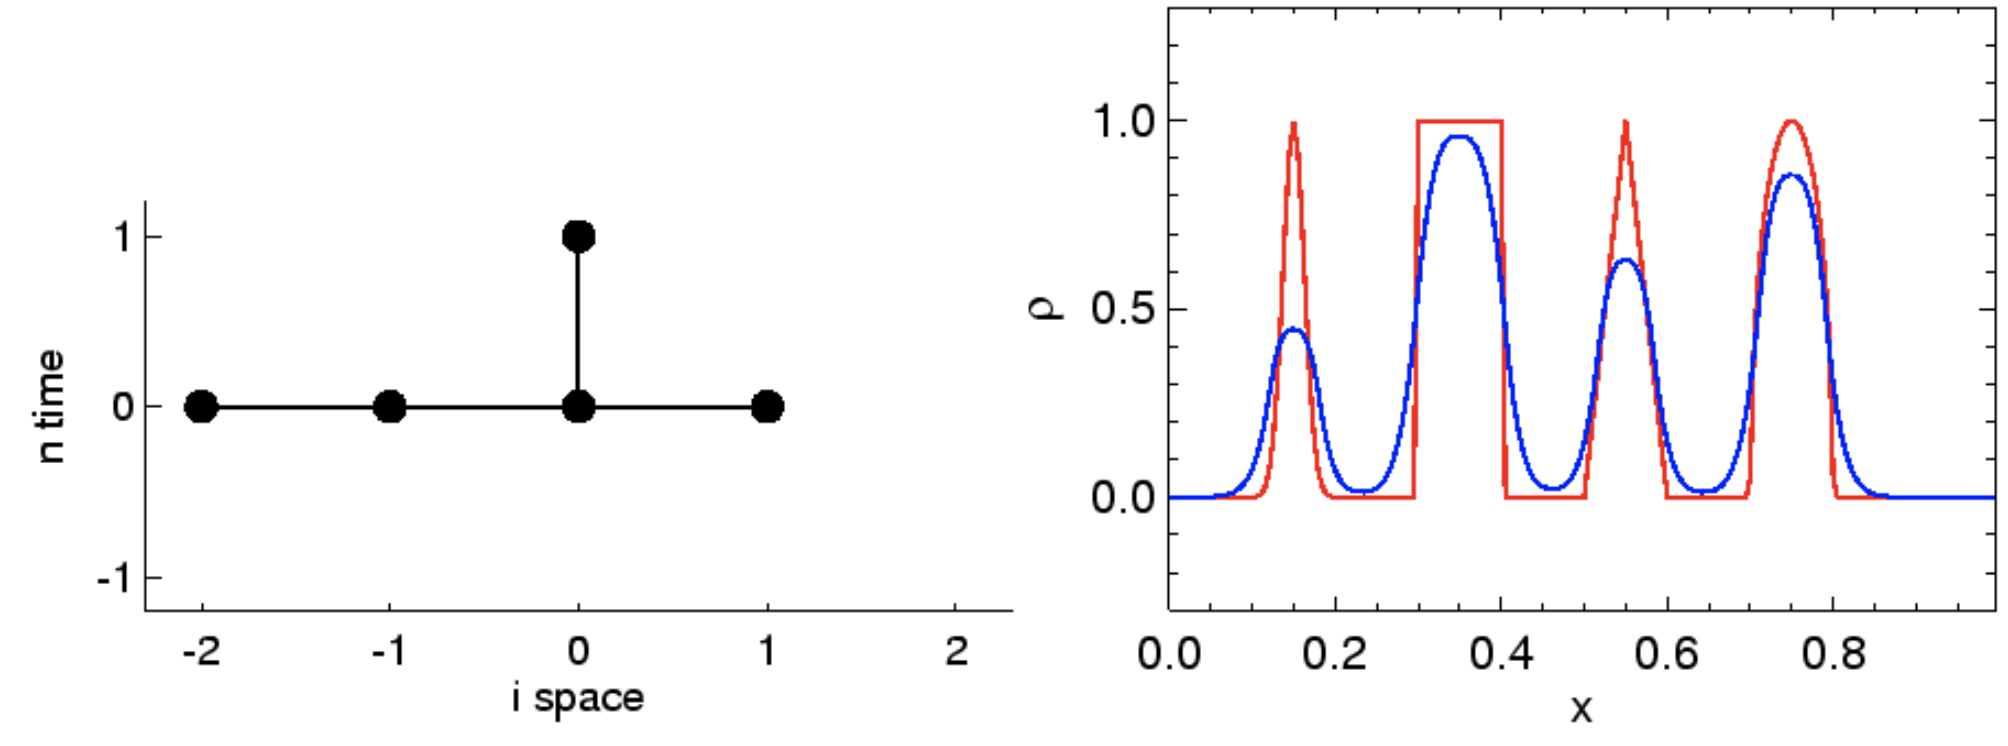
\includegraphics{./figs/minmod.png}}
  \end{center}
  \caption[]{Minmod}
  \label{fig:minmod}
\end{figure}

This method chooses the smallest of the two slopes, provided they both have the same sign, and
chooses 0 otherwise.

\subsubsection{Van Leer}

\begin{equation}
\delta q_i = \left\{
\begin{array}{ccc}
\frac{2}{\delta q_f^{-1} + \delta q_b^{-1}} & \quad & \mathrm{if} \quad \delta q_f \delta q_b > 0  \\
0 &\quad & \mathrm{if} \quad  \delta q_f \delta q_b \leq 0
\end{array}\right.
\end{equation}

\begin{figure}
  \begin{center}
    \resizebox{\textwidth}{!}{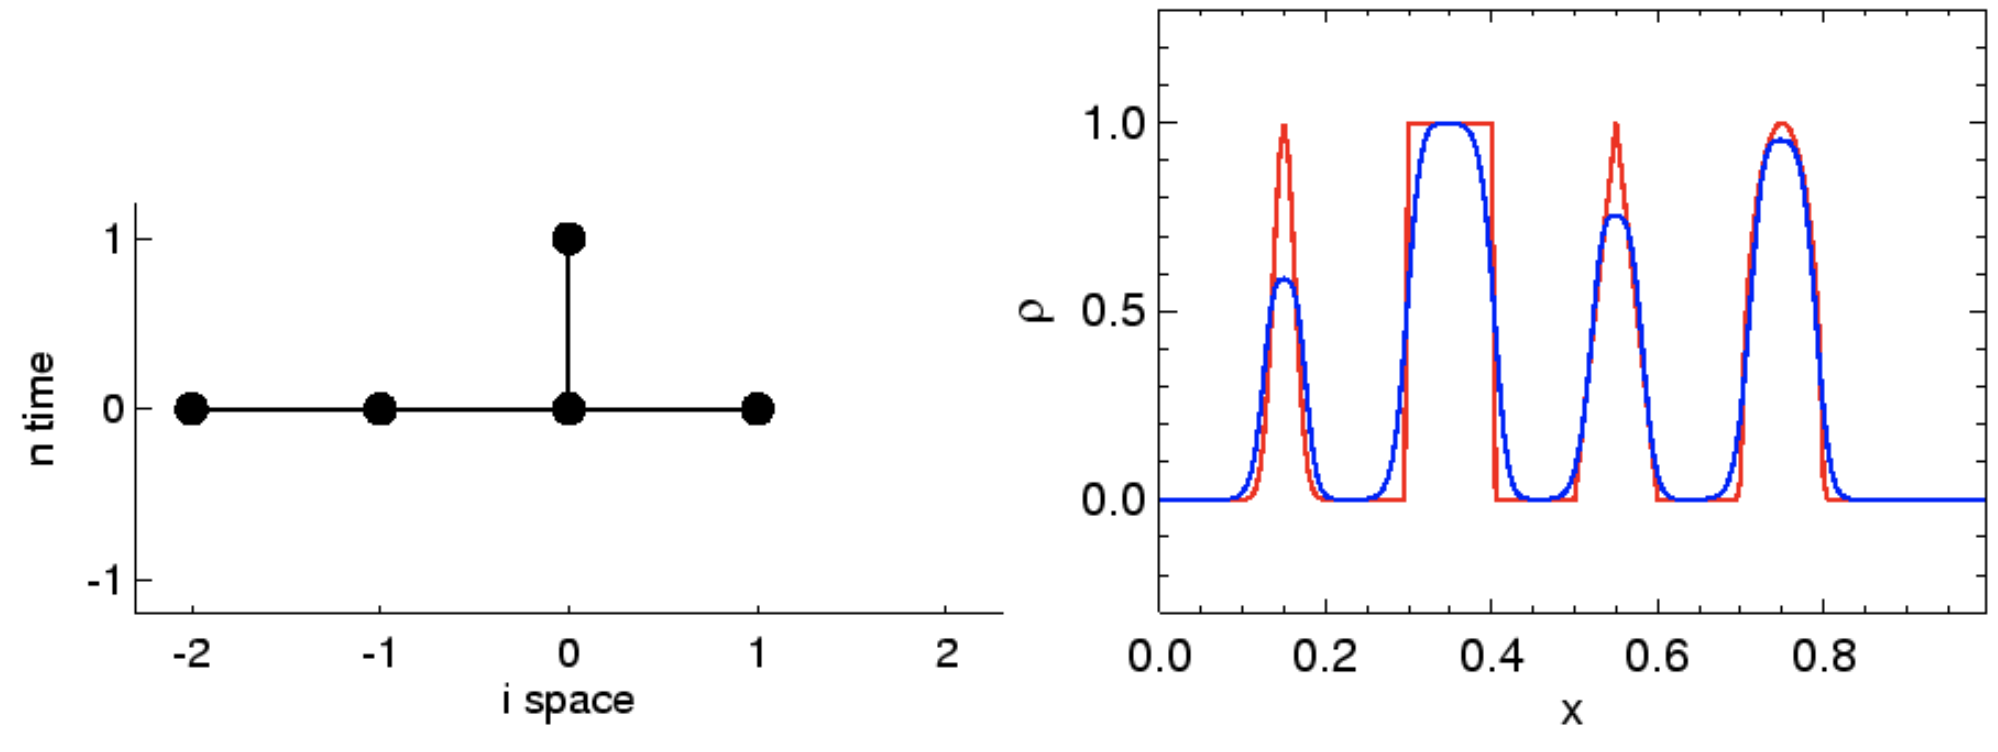
\includegraphics{./figs/vanleer.png}}
  \end{center}
  \caption[]{Van Leer}
  \label{fig:vanleer}
\end{figure}

\subsubsection{Superbee}

\begin{equation}
\delta q_i = \left[\mbox{sign}(\delta q_f) + \mbox{sign}(\delta q_b)\right] \times 
\mathrm{min} \left\{ \mbox{abs}(\delta q_f), \mbox{abs}(\delta q_b), \frac{1}{2} \mbox{max} \left[\mbox{abs}(\delta q_f),\mathrm{abs}\left(\delta q_b\right) \right]\right\}
\end{equation}


\begin{figure}
  \begin{center}
    \resizebox{\textwidth}{!}{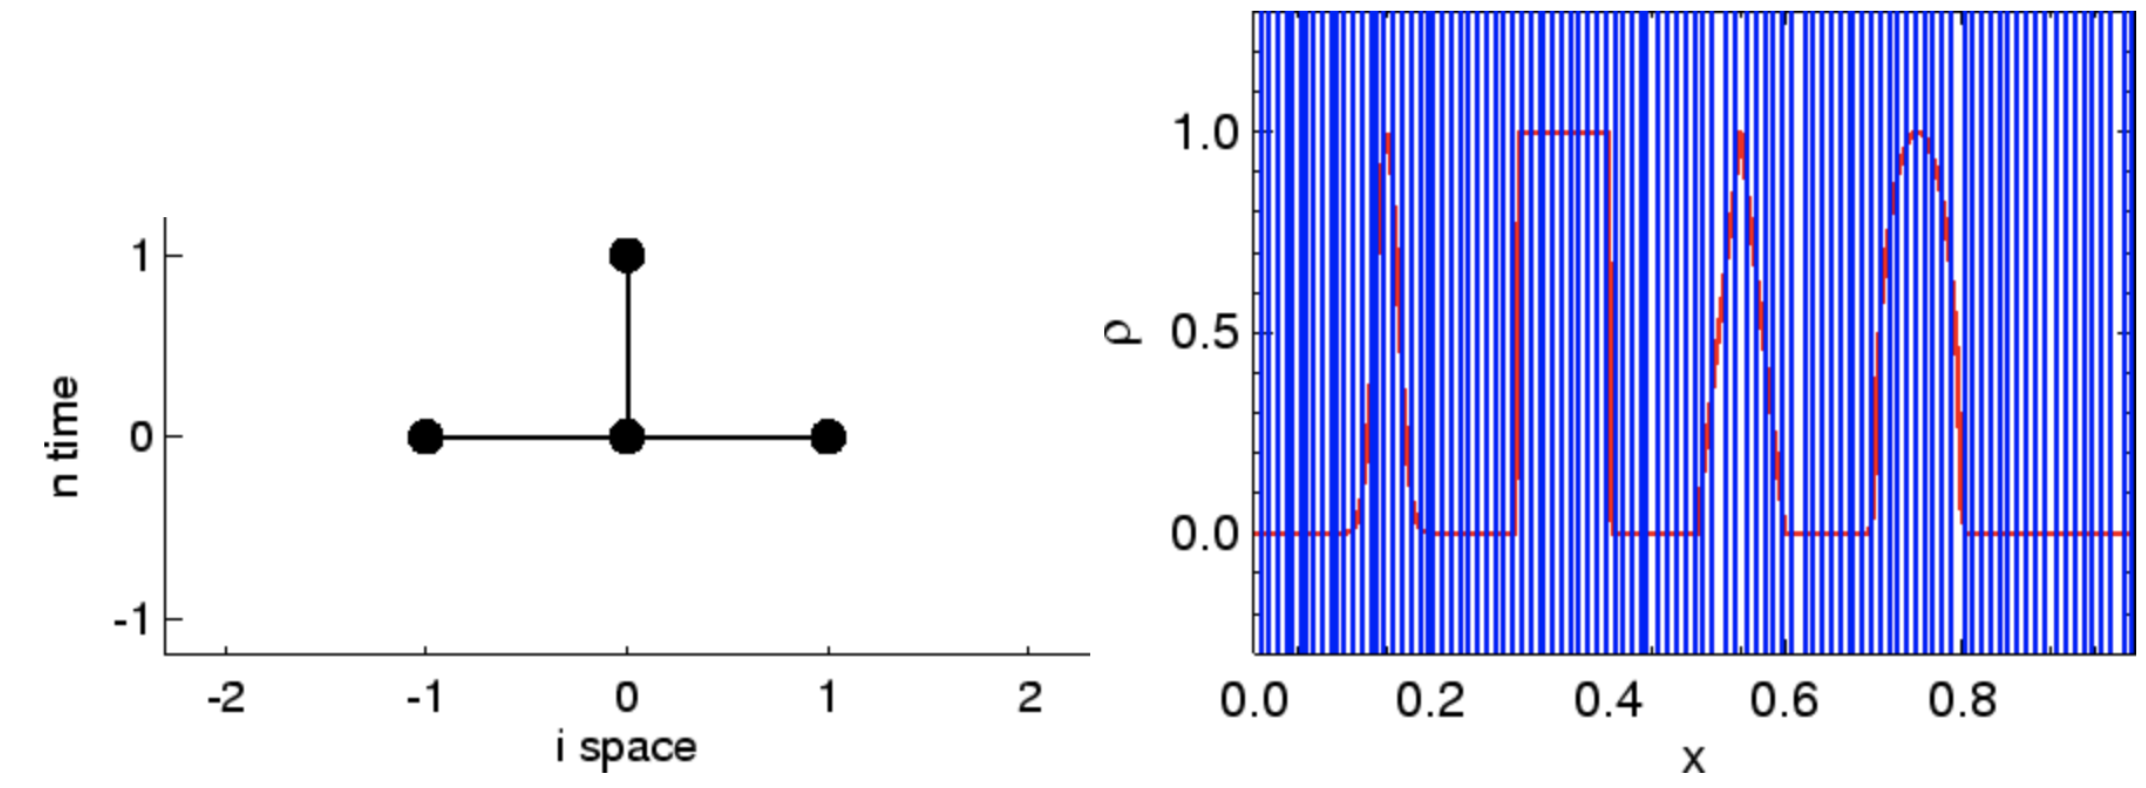
\includegraphics{./figs/superbee.png}}
  \end{center}
  \caption[]{Superbee}
  \label{fig:superbee}
\end{figure}

\subsection{Exercises}

\subsubsection{The stable schemes}

\begin{itemize}

\item Use a Gaussian ( $e^{-\left(x/0.1\right)^2}$) and a rectangle ( $1 \mbox{ for abs}(x) < 0.2 \mbox{ and } 0 \mbox{ elsewhere}$) as initial conditions. 

\item  Use a reasonable Courant number (e.g. $C=0.4$) and keep it fixed. Simulate a complete 
revolution ( $v\Delta T    = 1$) to facilitate the comparison with the exact final result (= initial condition).

\item  Compare the results for different resolutions (e.g. 25, 50, 100, 200 grid points).

\item  Measure the error with the following norms

\begin{itemize}
  
\item The 1-norm

\begin{equation}
N_1 = \frac{1}{N} \sum_i^N \mbox{abs}\left(q_i^{(t)} - q_i^{(0)}\right)
\end{equation}

\item The Euclidian 2-norm 

\begin{equation}
N_2 = \frac{1}{N} \left[\sum_i^N \mbox{abs}\left(q_i^{(t)} - q_i^{(0)}\right)^2\right]^{1/2}
\end{equation}

\item and the maximum-norm 


\begin{equation}
N_\mathrm{max} = \mbox{max abs} \left(q_i^{(t)} - q_i^{(0)}\right)
\end{equation}

\end{itemize}

\end{itemize}
